% \section{Combined system}
% \begin{frame}{Methods}{Combined System}	
% 		\begin{itemize}
% 			\item Input for control filter and CP
% 			\begin{itemize}
% 			\item $x[n]$
% 			\item $\hat{x}[n+P]$
% 			\end{itemize}
% 		\end{itemize}
% \begin{center}
% 	\resizebox{0.9\columnwidth}{!}{		
% 			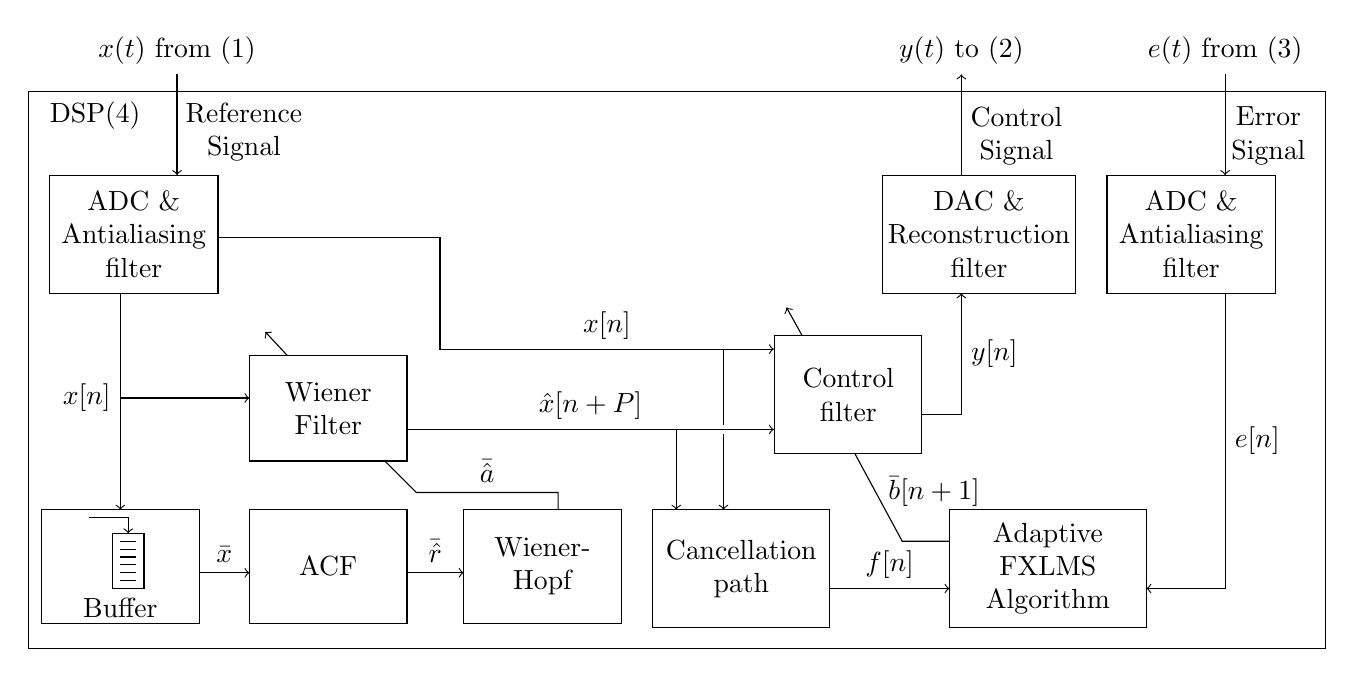
\begin{tikzpicture}
\draw  (-6.96,-2.17) rectangle node[text width=2cm,align=center] {ADC \& Antialiasing filter} (-4.82,-3.67);
\draw  (0.7,-6.42) rectangle node[text width=2.5cm,align=center] {Cancellation \\ path}(2.95,-7.92);
\draw  (4.47,-6.42) rectangle node[text width=2.5cm,align=center] {Adaptive FXLMS Algorithm} (6.97,-7.92);

\draw  (2.25,-4.21) rectangle node[text width=1.5cm,align=center,fill=white] {Control filter} (4.12,-5.71);
\draw  (3.62,-2.17) rectangle node[text width=2.5cm,align=center] {DAC \& \\ Reconstruction filter}(6.07,-3.67);
\draw  (6.47,-2.17) rectangle node[text width=2cm,align=center] {ADC \& Antialiasing filter}(8.61,-3.67);

\draw  (-7.23,-1.11) rectangle (9.25,-8.18);
\node at (-6.38,-1.41) {DSP(4)};
\node [text width=2cm,align=center] at (-4.49,-1.62) {Reference Signal};

\draw[->] (2.95,-7.42) -- node[above]{$f[n]$} (4.47,-7.42);

\draw[->] (7.97,-3.67) -- node[right]{$e[n]$} (7.97,-7.42)  -- (6.97,-7.42);

\draw [->](7.97,-0.89) node[above]{$e(t)$ from (3)} -- (7.97,-2.17) ;
\draw [->](4.62,-2.17)  --  (4.62,-0.89) node[above]{$y(t)$ to (2)};




\draw[->] (4.12,-5.21) -- (4.62,-5.21) --node[right]{$y[n]$} (4.62,-3.67);
\draw [->](-5.34,-0.89) node[above]{$x(t)$ from (1)} -- (-5.34,-2.17);
\node [text width=2cm,align=center] at (5.32,-1.67) {Control Signal};
\node [text width=1.5cm,align=center] at (8.52,-1.67) {Error Signal};

\draw (4.47,-6.82) -- (3.87,-6.82) --node[above=2.25,right]{$\bar{b}[n+1]$} (3.27,-5.71);
\draw [->](2.6,-4.21) -- (2.4,-3.85);


%% Boxes
\draw  (-4.42,-5.8) rectangle node[text width=2cm,align=center] {Wiener Filter}(-2.42,-4.46);
\draw  (-2.42,-6.42) rectangle node[text width=2cm,align=center] {ACF}(-4.42,-7.86);
\draw  (-5.06,-6.42) rectangle node[text width=2cm,align=center,below=8] {Buffer}(-7.06,-7.86);
\draw  (-1.7,-6.42) rectangle node[text width=1.5cm,align=center] {Wiener- Hopf}(0.3,-7.86);



%%Buffer
\draw (-5.76,-7.42) node (v1) {} -- (-6.16,-7.42) -- (-6.16,-6.72) -- (-5.76,-6.72) -- (-5.76,-7.42);
\draw (-6.06,-6.82) -- (-5.86,-6.82);
\draw (-6.06,-6.92) -- (-5.86,-6.92);
\draw (-6.06,-7.02) -- (-5.86,-7.02);
\draw (-6.06,-7.12) -- (-5.86,-7.12);
\draw (-6.06,-7.22) -- (-5.86,-7.22);
\draw (-6.06,-7.32) -- (-5.86,-7.32);
\draw [->](-6.46,-6.52) -- (-5.96,-6.52) -- (-5.96,-6.72);


%% Lines
\draw [->](-5.06,-7.22) -- node[above]{$\bar{x}$} (-4.42,-7.22);
\draw [->](-2.42,-7.22) -- node[above]{$\bar{\hat{r}}$}(-1.7,-7.22);
\draw (-0.5,-6.42) -- (-0.5,-6.2) -- node[above]{$\bar{\hat{a}}$} (-2.3,-6.2) -- (-2.7,-5.8);


\draw [->](-3.94,-4.46) -- (-4.22,-4.16);
\draw [->](-6.06,-5)  node[left]{$x[n]$} -- (-4.42,-5);
\draw [->](-6.06,-3.68) -- (-6.06,-6.42);
\draw [->](-2.42,-5.4) --  node[above]{$\hat{x}[n+P]$}(2.24,-5.4);

\draw [->](-4.82,-2.96) -- (-4.56,-2.96) -- (-2,-2.96) -- (-2,-4.38) -- node[above]{$x[n]$} (2.24,-4.38);
\draw (1.6,-4.38) -- (1.6,-5.34);
\draw [->](1.6,-5.46) -- (1.6,-6.42);
\draw [->](1,-5.4) -- (1,-6.42);
\end{tikzpicture}}
% \end{center}
% \end{frame}



\section{Simulations}
\subsection{How to test}

\begin{frame}{Simulation}{What to test?}	
\begin{itemize}
	\item Linear Prediction
	\begin{itemize}
		\item Optimal parameters for LP ($N$,$O$,$f_s$,$P$)
	\end{itemize}
	\item Feedforward FXLMS	
	\begin{itemize}
		\item Attenuation with different delays
		\item Frequency response
	\end{itemize}
\end{itemize}
\end{frame}

\begin{frame}{Simulation}{How to Test}	
\begin{itemize}
	\item Simulink
	\item Simulating with two systems 
	\begin{itemize}
		\item Linear Prediction
		\item Feedforward FXLMS
		\item Sound files are adapted 
	\end{itemize}
	\item Automation of simulations	
\end{itemize}
\end{frame}

\begin{frame}{Simulation}{How to Test}	
\begin{itemize}
	\item Archimedes Project (1992)
	\item Well known speech signal
	\item $f_s = 44.1$ [kHz] 
	\item Measured in anechoic chamber		
\end{itemize}
\end{frame}


% \begin{frame}{Simulation Results}{Analysis of results}	
% \begin{itemize}
% 	\item Linear Prediction
% 	\begin{itemize}
% 		\item Prediction Gain: $PG = 10 log_{10}\bigg(\frac{\sigma^2_x}{\sigma^2_\varepsilon}\bigg) = 10 log_{10}\bigg(\frac{E\{x^2[n]\}}{E\{\varepsilon^2[n]\}}\bigg)$
% 	\end{itemize}
% 	\item Feedforward FXLMS
% 	\begin{itemize}
% 		\item Filter-bank
% 	\end{itemize}
% \end{itemize}
% \end{frame}


\subsection{Linear Prediction Parameters}
\begin{frame}{Simulation Results}{Optimal parameters}		
\begin{columns}
	\begin{column}{0.4\textwidth}
		\begin{itemize}
			\item Prediction order P = 43
			\item Optimal parameters
			\begin{itemize}
				\item Framelength N = 1600
				\item Overlap O = 1500
			\end{itemize}
			\item Prediction Gain PG = 5.4 dB
		\end{itemize}
	\end{column}
	\begin{column}{0.6\textwidth} 
		\resizebox{0.9\columnwidth}{!}{		
			% This file was created by matlab2tikz.
%
%The latest updates can be retrieved from
%  http://www.mathworks.com/matlabcentral/fileexchange/22022-matlab2tikz-matlab2tikz
%where you can also make suggestions and rate matlab2tikz.
%
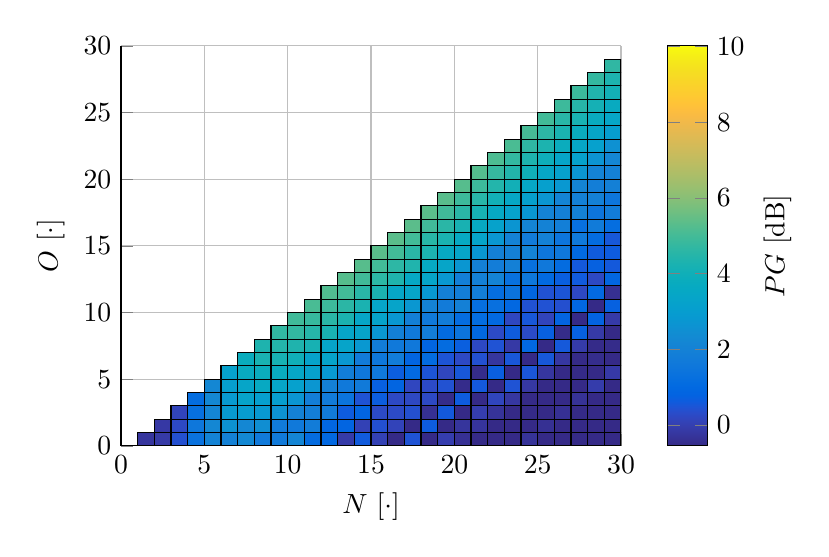
\begin{tikzpicture}


\begin{axis}[%
width=2.5in,
height=2in,
scale only axis,
point meta min=-0.551769511455843,
point meta max=10.0207598959184,
unbounded coords=jump,
xmin=0,
xmax=3000,
xlabel={$N$ [$\cdot$]},
xmajorgrids,
ymin=0,
ymax=3000,
ytick={0,500,...,3000},
yticklabels={0,5,...,30},
xtick={0,500,...,3000},
xticklabels={0,5,...,30},
ylabel={$O$ [$\cdot$]},
ymajorgrids,
axis background/.style={fill=white},
axis x line*=bottom,
axis y line*=left,
colormap={mymap}{[1pt] rgb(0pt)=(0.2081,0.1663,0.5292); rgb(1pt)=(0.211624,0.189781,0.577676); rgb(2pt)=(0.212252,0.213771,0.626971); rgb(3pt)=(0.2081,0.2386,0.677086); rgb(4pt)=(0.195905,0.264457,0.7279); rgb(5pt)=(0.170729,0.291938,0.779248); rgb(6pt)=(0.125271,0.324243,0.830271); rgb(7pt)=(0.0591333,0.359833,0.868333); rgb(8pt)=(0.0116952,0.38751,0.881957); rgb(9pt)=(0.00595714,0.408614,0.882843); rgb(10pt)=(0.0165143,0.4266,0.878633); rgb(11pt)=(0.0328524,0.443043,0.871957); rgb(12pt)=(0.0498143,0.458571,0.864057); rgb(13pt)=(0.0629333,0.47369,0.855438); rgb(14pt)=(0.0722667,0.488667,0.8467); rgb(15pt)=(0.0779429,0.503986,0.838371); rgb(16pt)=(0.0793476,0.520024,0.831181); rgb(17pt)=(0.0749429,0.537543,0.826271); rgb(18pt)=(0.0640571,0.556986,0.823957); rgb(19pt)=(0.0487714,0.577224,0.822829); rgb(20pt)=(0.0343429,0.596581,0.819852); rgb(21pt)=(0.0265,0.6137,0.8135); rgb(22pt)=(0.0238905,0.628662,0.803762); rgb(23pt)=(0.0230905,0.641786,0.791267); rgb(24pt)=(0.0227714,0.653486,0.776757); rgb(25pt)=(0.0266619,0.664195,0.760719); rgb(26pt)=(0.0383714,0.674271,0.743552); rgb(27pt)=(0.0589714,0.683757,0.725386); rgb(28pt)=(0.0843,0.692833,0.706167); rgb(29pt)=(0.113295,0.7015,0.685857); rgb(30pt)=(0.145271,0.709757,0.664629); rgb(31pt)=(0.180133,0.717657,0.642433); rgb(32pt)=(0.217829,0.725043,0.619262); rgb(33pt)=(0.258643,0.731714,0.595429); rgb(34pt)=(0.302171,0.737605,0.571186); rgb(35pt)=(0.348167,0.742433,0.547267); rgb(36pt)=(0.395257,0.7459,0.524443); rgb(37pt)=(0.44201,0.748081,0.503314); rgb(38pt)=(0.487124,0.749062,0.483976); rgb(39pt)=(0.530029,0.749114,0.466114); rgb(40pt)=(0.570857,0.748519,0.44939); rgb(41pt)=(0.609852,0.747314,0.433686); rgb(42pt)=(0.6473,0.7456,0.4188); rgb(43pt)=(0.683419,0.743476,0.404433); rgb(44pt)=(0.71841,0.741133,0.390476); rgb(45pt)=(0.752486,0.7384,0.376814); rgb(46pt)=(0.785843,0.735567,0.363271); rgb(47pt)=(0.818505,0.732733,0.34979); rgb(48pt)=(0.850657,0.7299,0.336029); rgb(49pt)=(0.882433,0.727433,0.3217); rgb(50pt)=(0.913933,0.725786,0.306276); rgb(51pt)=(0.944957,0.726114,0.288643); rgb(52pt)=(0.973895,0.731395,0.266648); rgb(53pt)=(0.993771,0.745457,0.240348); rgb(54pt)=(0.999043,0.765314,0.216414); rgb(55pt)=(0.995533,0.786057,0.196652); rgb(56pt)=(0.988,0.8066,0.179367); rgb(57pt)=(0.978857,0.827143,0.163314); rgb(58pt)=(0.9697,0.848138,0.147452); rgb(59pt)=(0.962586,0.870514,0.1309); rgb(60pt)=(0.958871,0.8949,0.113243); rgb(61pt)=(0.959824,0.921833,0.0948381); rgb(62pt)=(0.9661,0.951443,0.0755333); rgb(63pt)=(0.9763,0.9831,0.0538)},
colorbar,
colorbar style={ylabel={$PG$ [dB]}}
]

\addplot[%
surf,
shader=flat corner,draw=black,colormap={mymap}{[1pt] rgb(0pt)=(0.2081,0.1663,0.5292); rgb(1pt)=(0.211624,0.189781,0.577676); rgb(2pt)=(0.212252,0.213771,0.626971); rgb(3pt)=(0.2081,0.2386,0.677086); rgb(4pt)=(0.195905,0.264457,0.7279); rgb(5pt)=(0.170729,0.291938,0.779248); rgb(6pt)=(0.125271,0.324243,0.830271); rgb(7pt)=(0.0591333,0.359833,0.868333); rgb(8pt)=(0.0116952,0.38751,0.881957); rgb(9pt)=(0.00595714,0.408614,0.882843); rgb(10pt)=(0.0165143,0.4266,0.878633); rgb(11pt)=(0.0328524,0.443043,0.871957); rgb(12pt)=(0.0498143,0.458571,0.864057); rgb(13pt)=(0.0629333,0.47369,0.855438); rgb(14pt)=(0.0722667,0.488667,0.8467); rgb(15pt)=(0.0779429,0.503986,0.838371); rgb(16pt)=(0.0793476,0.520024,0.831181); rgb(17pt)=(0.0749429,0.537543,0.826271); rgb(18pt)=(0.0640571,0.556986,0.823957); rgb(19pt)=(0.0487714,0.577224,0.822829); rgb(20pt)=(0.0343429,0.596581,0.819852); rgb(21pt)=(0.0265,0.6137,0.8135); rgb(22pt)=(0.0238905,0.628662,0.803762); rgb(23pt)=(0.0230905,0.641786,0.791267); rgb(24pt)=(0.0227714,0.653486,0.776757); rgb(25pt)=(0.0266619,0.664195,0.760719); rgb(26pt)=(0.0383714,0.674271,0.743552); rgb(27pt)=(0.0589714,0.683757,0.725386); rgb(28pt)=(0.0843,0.692833,0.706167); rgb(29pt)=(0.113295,0.7015,0.685857); rgb(30pt)=(0.145271,0.709757,0.664629); rgb(31pt)=(0.180133,0.717657,0.642433); rgb(32pt)=(0.217829,0.725043,0.619262); rgb(33pt)=(0.258643,0.731714,0.595429); rgb(34pt)=(0.302171,0.737605,0.571186); rgb(35pt)=(0.348167,0.742433,0.547267); rgb(36pt)=(0.395257,0.7459,0.524443); rgb(37pt)=(0.44201,0.748081,0.503314); rgb(38pt)=(0.487124,0.749062,0.483976); rgb(39pt)=(0.530029,0.749114,0.466114); rgb(40pt)=(0.570857,0.748519,0.44939); rgb(41pt)=(0.609852,0.747314,0.433686); rgb(42pt)=(0.6473,0.7456,0.4188); rgb(43pt)=(0.683419,0.743476,0.404433); rgb(44pt)=(0.71841,0.741133,0.390476); rgb(45pt)=(0.752486,0.7384,0.376814); rgb(46pt)=(0.785843,0.735567,0.363271); rgb(47pt)=(0.818505,0.732733,0.34979); rgb(48pt)=(0.850657,0.7299,0.336029); rgb(49pt)=(0.882433,0.727433,0.3217); rgb(50pt)=(0.913933,0.725786,0.306276); rgb(51pt)=(0.944957,0.726114,0.288643); rgb(52pt)=(0.973895,0.731395,0.266648); rgb(53pt)=(0.993771,0.745457,0.240348); rgb(54pt)=(0.999043,0.765314,0.216414); rgb(55pt)=(0.995533,0.786057,0.196652); rgb(56pt)=(0.988,0.8066,0.179367); rgb(57pt)=(0.978857,0.827143,0.163314); rgb(58pt)=(0.9697,0.848138,0.147452); rgb(59pt)=(0.962586,0.870514,0.1309); rgb(60pt)=(0.958871,0.8949,0.113243); rgb(61pt)=(0.959824,0.921833,0.0948381); rgb(62pt)=(0.9661,0.951443,0.0755333); rgb(63pt)=(0.9763,0.9831,0.0538)},mesh/rows=30]
table[row sep=crcr, point meta=\thisrow{c}] {%
	%
	x	y	c\\
	100	0	-0.249851110691807\\
	100	100	nan\\
	100	200	nan\\
	100	300	nan\\
	100	400	nan\\
	100	500	nan\\
	100	600	nan\\
	100	700	nan\\
	100	800	nan\\
	100	900	nan\\
	100	1000	nan\\
	100	1100	nan\\
	100	1200	nan\\
	100	1300	nan\\
	100	1400	nan\\
	100	1500	nan\\
	100	1600	nan\\
	100	1700	nan\\
	100	1800	nan\\
	100	1900	nan\\
	100	2000	nan\\
	100	2100	nan\\
	100	2200	nan\\
	100	2300	nan\\
	100	2400	nan\\
	100	2500	nan\\
	100	2600	nan\\
	100	2700	nan\\
	100	2800	nan\\
	100	2900	nan\\
	200	0	-0.134212977797894\\
	200	100	-0.167103642187056\\
	200	200	nan\\
	200	300	nan\\
	200	400	nan\\
	200	500	nan\\
	200	600	nan\\
	200	700	nan\\
	200	800	nan\\
	200	900	nan\\
	200	1000	nan\\
	200	1100	nan\\
	200	1200	nan\\
	200	1300	nan\\
	200	1400	nan\\
	200	1500	nan\\
	200	1600	nan\\
	200	1700	nan\\
	200	1800	nan\\
	200	1900	nan\\
	200	2000	nan\\
	200	2100	nan\\
	200	2200	nan\\
	200	2300	nan\\
	200	2400	nan\\
	200	2500	nan\\
	200	2600	nan\\
	200	2700	nan\\
	200	2800	nan\\
	200	2900	nan\\
	300	0	0.40073258158409\\
	300	100	0.251927782024709\\
	300	200	0.142801564300892\\
	300	300	nan\\
	300	400	nan\\
	300	500	nan\\
	300	600	nan\\
	300	700	nan\\
	300	800	nan\\
	300	900	nan\\
	300	1000	nan\\
	300	1100	nan\\
	300	1200	nan\\
	300	1300	nan\\
	300	1400	nan\\
	300	1500	nan\\
	300	1600	nan\\
	300	1700	nan\\
	300	1800	nan\\
	300	1900	nan\\
	300	2000	nan\\
	300	2100	nan\\
	300	2200	nan\\
	300	2300	nan\\
	300	2400	nan\\
	300	2500	nan\\
	300	2600	nan\\
	300	2700	nan\\
	300	2800	nan\\
	300	2900	nan\\
	400	0	1.35498518276026\\
	400	100	1.54062929586375\\
	400	200	1.25091430573651\\
	400	300	1.13011541776478\\
	400	400	nan\\
	400	500	nan\\
	400	600	nan\\
	400	700	nan\\
	400	800	nan\\
	400	900	nan\\
	400	1000	nan\\
	400	1100	nan\\
	400	1200	nan\\
	400	1300	nan\\
	400	1400	nan\\
	400	1500	nan\\
	400	1600	nan\\
	400	1700	nan\\
	400	1800	nan\\
	400	1900	nan\\
	400	2000	nan\\
	400	2100	nan\\
	400	2200	nan\\
	400	2300	nan\\
	400	2400	nan\\
	400	2500	nan\\
	400	2600	nan\\
	400	2700	nan\\
	400	2800	nan\\
	400	2900	nan\\
	500	0	2.07613030072784\\
	500	100	2.23484268450241\\
	500	200	2.16667780407076\\
	500	300	2.22280459708376\\
	500	400	2.22773910206715\\
	500	500	nan\\
	500	600	nan\\
	500	700	nan\\
	500	800	nan\\
	500	900	nan\\
	500	1000	nan\\
	500	1100	nan\\
	500	1200	nan\\
	500	1300	nan\\
	500	1400	nan\\
	500	1500	nan\\
	500	1600	nan\\
	500	1700	nan\\
	500	1800	nan\\
	500	1900	nan\\
	500	2000	nan\\
	500	2100	nan\\
	500	2200	nan\\
	500	2300	nan\\
	500	2400	nan\\
	500	2500	nan\\
	500	2600	nan\\
	500	2700	nan\\
	500	2800	nan\\
	500	2900	nan\\
	600	0	2.0053564589082\\
	600	100	2.61259722918176\\
	600	200	2.8832092344045\\
	600	300	2.86284941749047\\
	600	400	3.10314445957564\\
	600	500	3.19779941497919\\
	600	600	nan\\
	600	700	nan\\
	600	800	nan\\
	600	900	nan\\
	600	1000	nan\\
	600	1100	nan\\
	600	1200	nan\\
	600	1300	nan\\
	600	1400	nan\\
	600	1500	nan\\
	600	1600	nan\\
	600	1700	nan\\
	600	1800	nan\\
	600	1900	nan\\
	600	2000	nan\\
	600	2100	nan\\
	600	2200	nan\\
	600	2300	nan\\
	600	2400	nan\\
	600	2500	nan\\
	600	2600	nan\\
	600	2700	nan\\
	600	2800	nan\\
	600	2900	nan\\
	700	0	2.2744146608244\\
	700	100	2.21229720700257\\
	700	200	2.93838458205897\\
	700	300	3.29709652218325\\
	700	400	3.37210041995159\\
	700	500	3.73517577501174\\
	700	600	3.8204270648783\\
	700	700	nan\\
	700	800	nan\\
	700	900	nan\\
	700	1000	nan\\
	700	1100	nan\\
	700	1200	nan\\
	700	1300	nan\\
	700	1400	nan\\
	700	1500	nan\\
	700	1600	nan\\
	700	1700	nan\\
	700	1800	nan\\
	700	1900	nan\\
	700	2000	nan\\
	700	2100	nan\\
	700	2200	nan\\
	700	2300	nan\\
	700	2400	nan\\
	700	2500	nan\\
	700	2600	nan\\
	700	2700	nan\\
	700	2800	nan\\
	700	2900	nan\\
	800	0	1.6764398517674\\
	800	100	2.47790908751089\\
	800	200	2.84811066063823\\
	800	300	3.0687707331656\\
	800	400	3.63876502838183\\
	800	500	3.84993979572264\\
	800	600	4.22707612972411\\
	800	700	4.34417470624987\\
	800	800	nan\\
	800	900	nan\\
	800	1000	nan\\
	800	1100	nan\\
	800	1200	nan\\
	800	1300	nan\\
	800	1400	nan\\
	800	1500	nan\\
	800	1600	nan\\
	800	1700	nan\\
	800	1800	nan\\
	800	1900	nan\\
	800	2000	nan\\
	800	2100	nan\\
	800	2200	nan\\
	800	2300	nan\\
	800	2400	nan\\
	800	2500	nan\\
	800	2600	nan\\
	800	2700	nan\\
	800	2800	nan\\
	800	2900	nan\\
	900	0	1.6957478568352\\
	900	100	1.7319915851467\\
	900	200	2.60512775573002\\
	900	300	2.98481824622671\\
	900	400	3.37091511369957\\
	900	500	3.74946849304965\\
	900	600	4.17472244368776\\
	900	700	4.46545647083027\\
	900	800	4.70107297446204\\
	900	900	nan\\
	900	1000	nan\\
	900	1100	nan\\
	900	1200	nan\\
	900	1300	nan\\
	900	1400	nan\\
	900	1500	nan\\
	900	1600	nan\\
	900	1700	nan\\
	900	1800	nan\\
	900	1900	nan\\
	900	2000	nan\\
	900	2100	nan\\
	900	2200	nan\\
	900	2300	nan\\
	900	2400	nan\\
	900	2500	nan\\
	900	2600	nan\\
	900	2700	nan\\
	900	2800	nan\\
	900	2900	nan\\
	1000	0	2.14279356476327\\
	1000	100	1.65662756562456\\
	1000	200	1.9975093051342\\
	1000	300	2.68811548919998\\
	1000	400	3.15564116436878\\
	1000	500	3.43923191192347\\
	1000	600	4.00698906883707\\
	1000	700	4.36135318968568\\
	1000	800	4.71880877909074\\
	1000	900	4.9493889064919\\
	1000	1000	nan\\
	1000	1100	nan\\
	1000	1200	nan\\
	1000	1300	nan\\
	1000	1400	nan\\
	1000	1500	nan\\
	1000	1600	nan\\
	1000	1700	nan\\
	1000	1800	nan\\
	1000	1900	nan\\
	1000	2000	nan\\
	1000	2100	nan\\
	1000	2200	nan\\
	1000	2300	nan\\
	1000	2400	nan\\
	1000	2500	nan\\
	1000	2600	nan\\
	1000	2700	nan\\
	1000	2800	nan\\
	1000	2900	nan\\
	1100	0	1.08628380389681\\
	1100	100	1.78373115008797\\
	1100	200	1.83869495569938\\
	1100	300	1.84921642836682\\
	1100	400	2.72090762354963\\
	1100	500	3.19932951902192\\
	1100	600	3.28763346728818\\
	1100	700	4.1733005127402\\
	1100	800	4.49383265009054\\
	1100	900	4.81677388898654\\
	1100	1000	5.09223132392375\\
	1100	1100	nan\\
	1100	1200	nan\\
	1100	1300	nan\\
	1100	1400	nan\\
	1100	1500	nan\\
	1100	1600	nan\\
	1100	1700	nan\\
	1100	1800	nan\\
	1100	1900	nan\\
	1100	2000	nan\\
	1100	2100	nan\\
	1100	2200	nan\\
	1100	2300	nan\\
	1100	2400	nan\\
	1100	2500	nan\\
	1100	2600	nan\\
	1100	2700	nan\\
	1100	2800	nan\\
	1100	2900	nan\\
	1200	0	0.96228292179036\\
	1200	100	0.874714526881095\\
	1200	200	1.74822965859813\\
	1200	300	1.74613873946482\\
	1200	400	1.96406088862939\\
	1200	500	2.83528036765025\\
	1200	600	3.27582233051984\\
	1200	700	3.34225172739605\\
	1200	800	4.2270814155954\\
	1200	900	4.5852271687131\\
	1200	1000	4.90782372375419\\
	1200	1100	5.19666553372495\\
	1200	1200	nan\\
	1200	1300	nan\\
	1200	1400	nan\\
	1200	1500	nan\\
	1200	1600	nan\\
	1200	1700	nan\\
	1200	1800	nan\\
	1200	1900	nan\\
	1200	2000	nan\\
	1200	2100	nan\\
	1200	2200	nan\\
	1200	2300	nan\\
	1200	2400	nan\\
	1200	2500	nan\\
	1200	2600	nan\\
	1200	2700	nan\\
	1200	2800	nan\\
	1200	2900	nan\\
	1300	0	-0.107030717223719\\
	1300	100	0.850232560605215\\
	1300	200	0.637949811893221\\
	1300	300	1.40384792467279\\
	1300	400	1.64958254277473\\
	1300	500	1.79741249348277\\
	1300	600	2.75608764238935\\
	1300	700	3.32534859240284\\
	1300	800	3.40167471419125\\
	1300	900	4.26932143570372\\
	1300	1000	4.60365364811444\\
	1300	1100	4.98195949948451\\
	1300	1200	5.28042149364273\\
	1300	1300	nan\\
	1300	1400	nan\\
	1300	1500	nan\\
	1300	1600	nan\\
	1300	1700	nan\\
	1300	1800	nan\\
	1300	1900	nan\\
	1300	2000	nan\\
	1300	2100	nan\\
	1300	2200	nan\\
	1300	2300	nan\\
	1300	2400	nan\\
	1300	2500	nan\\
	1300	2600	nan\\
	1300	2700	nan\\
	1300	2800	nan\\
	1300	2900	nan\\
	1400	0	0.601907313869925\\
	1400	100	0.0657729838043244\\
	1400	200	0.862145199127073\\
	1400	300	0.460707580490794\\
	1400	400	1.68525830954437\\
	1400	500	1.55802793388997\\
	1400	600	1.74594940231651\\
	1400	700	2.81551743753557\\
	1400	800	3.32371598632194\\
	1400	900	3.42520085860678\\
	1400	1000	4.25956377468848\\
	1400	1100	4.56477323219294\\
	1400	1200	4.97384046578701\\
	1400	1300	5.29633096641679\\
	1400	1400	nan\\
	1400	1500	nan\\
	1400	1600	nan\\
	1400	1700	nan\\
	1400	1800	nan\\
	1400	1900	nan\\
	1400	2000	nan\\
	1400	2100	nan\\
	1400	2200	nan\\
	1400	2300	nan\\
	1400	2400	nan\\
	1400	2500	nan\\
	1400	2600	nan\\
	1400	2700	nan\\
	1400	2800	nan\\
	1400	2900	nan\\
	1500	0	0.0479688920623348\\
	1500	100	0.409815317960011\\
	1500	200	0.265969244574455\\
	1500	300	0.66329040490881\\
	1500	400	0.725248934820509\\
	1500	500	1.62075499462296\\
	1500	600	1.53068266641447\\
	1500	700	1.78380983455356\\
	1500	800	2.75223306087479\\
	1500	900	3.29361894997763\\
	1500	1000	3.36423431504327\\
	1500	1100	4.28085176540069\\
	1500	1200	4.61221553749839\\
	1500	1300	4.99326970538795\\
	1500	1400	5.32976716671813\\
	1500	1500	nan\\
	1500	1600	nan\\
	1500	1700	nan\\
	1500	1800	nan\\
	1500	1900	nan\\
	1500	2000	nan\\
	1500	2100	nan\\
	1500	2200	nan\\
	1500	2300	nan\\
	1500	2400	nan\\
	1500	2500	nan\\
	1500	2600	nan\\
	1500	2700	nan\\
	1500	2800	nan\\
	1500	2900	nan\\
	1600	0	-0.605169389430681\\
	1600	100	0.117420548822926\\
	1600	200	0.284797641762555\\
	1600	300	0.253253520189372\\
	1600	400	0.870129979674615\\
	1600	500	0.671127168444688\\
	1600	600	1.74986538278574\\
	1600	700	1.64439306142093\\
	1600	800	1.91148110154675\\
	1600	900	2.77573952375898\\
	1600	1000	3.32540102344824\\
	1600	1100	3.44971766694812\\
	1600	1200	4.36003073667673\\
	1600	1300	4.62738934446695\\
	1600	1400	4.98723836519226\\
	1600	1500	5.34050250023747\\
	1600	1600	nan\\
	1600	1700	nan\\
	1600	1800	nan\\
	1600	1900	nan\\
	1600	2000	nan\\
	1600	2100	nan\\
	1600	2200	nan\\
	1600	2300	nan\\
	1600	2400	nan\\
	1600	2500	nan\\
	1600	2600	nan\\
	1600	2700	nan\\
	1600	2800	nan\\
	1600	2900	nan\\
	1700	0	0.459481577183121\\
	1700	100	-0.828238464808588\\
	1700	200	0.392172946743951\\
	1700	300	0.226384351456075\\
	1700	400	0.183454984733797\\
	1700	500	1.03300677343369\\
	1700	600	0.866722268193889\\
	1700	700	1.60939528933199\\
	1700	800	1.64458351852261\\
	1700	900	1.91984952325872\\
	1700	1000	2.75640854387435\\
	1700	1100	3.37358423554233\\
	1700	1200	3.57831957034059\\
	1700	1300	4.38037462195002\\
	1700	1400	4.57895857617312\\
	1700	1500	4.99333526811925\\
	1700	1600	5.35096269740123\\
	1700	1700	nan\\
	1700	1800	nan\\
	1700	1900	nan\\
	1700	2000	nan\\
	1700	2100	nan\\
	1700	2200	nan\\
	1700	2300	nan\\
	1700	2400	nan\\
	1700	2500	nan\\
	1700	2600	nan\\
	1700	2700	nan\\
	1700	2800	nan\\
	1700	2900	nan\\
	1800	0	-1.41853543923144\\
	1800	100	0.632649966343857\\
	1800	200	-0.384497042533314\\
	1800	300	0.255556860908392\\
	1800	400	0.286777052802089\\
	1800	500	0.482107568083193\\
	1800	600	1.07739734854062\\
	1800	700	0.851941681167397\\
	1800	800	1.82437185471004\\
	1800	900	1.65998697525295\\
	1800	1000	2.01342546713771\\
	1800	1100	2.84347279090459\\
	1800	1200	3.39849928401779\\
	1800	1300	3.59204978113913\\
	1800	1400	4.2917812700128\\
	1800	1500	4.54262260148609\\
	1800	1600	4.9656993136051\\
	1800	1700	5.33339229740171\\
	1800	1800	nan\\
	1800	1900	nan\\
	1800	2000	nan\\
	1800	2100	nan\\
	1800	2200	nan\\
	1800	2300	nan\\
	1800	2400	nan\\
	1800	2500	nan\\
	1800	2600	nan\\
	1800	2700	nan\\
	1800	2800	nan\\
	1800	2900	nan\\
	1900	0	-0.0337222813430315\\
	1900	100	-1.17881791521385\\
	1900	200	0.579738688002559\\
	1900	300	-0.504820413080548\\
	1900	400	0.43222545991656\\
	1900	500	0.172356634139464\\
	1900	600	0.486159910021189\\
	1900	700	1.08979803776635\\
	1900	800	1.06421189967321\\
	1900	900	1.76198646065506\\
	1900	1000	1.73893709942167\\
	1900	1100	1.94136948935232\\
	1900	1200	2.79511100023429\\
	1900	1300	3.40973957807585\\
	1900	1400	3.5985713113068\\
	1900	1500	4.25686359222365\\
	1900	1600	4.58134558875467\\
	1900	1700	4.95173298101252\\
	1900	1800	5.32121533683218\\
	1900	1900	nan\\
	1900	2000	nan\\
	1900	2100	nan\\
	1900	2200	nan\\
	1900	2300	nan\\
	1900	2400	nan\\
	1900	2500	nan\\
	1900	2600	nan\\
	1900	2700	nan\\
	1900	2800	nan\\
	1900	2900	nan\\
	2000	0	-0.38106458141862\\
	2000	100	-0.265003051545396\\
	2000	200	-1.23043392090561\\
	2000	300	0.636229173175987\\
	2000	400	-0.501393709183734\\
	2000	500	0.531105328460703\\
	2000	600	0.24654842554858\\
	2000	700	0.693751402870032\\
	2000	800	1.42643544661484\\
	2000	900	1.14002253653198\\
	2000	1000	1.9301916384988\\
	2000	1100	1.86037182253522\\
	2000	1200	1.89839206221938\\
	2000	1300	2.74843083934798\\
	2000	1400	3.37740852093157\\
	2000	1500	3.61406316805146\\
	2000	1600	4.20147952106818\\
	2000	1700	4.57501484363941\\
	2000	1800	4.91198130207837\\
	2000	1900	5.28767930948696\\
	2000	2000	nan\\
	2000	2100	nan\\
	2000	2200	nan\\
	2000	2300	nan\\
	2000	2400	nan\\
	2000	2500	nan\\
	2000	2600	nan\\
	2000	2700	nan\\
	2000	2800	nan\\
	2000	2900	nan\\
	2100	0	-2.54778888937748\\
	2100	100	-0.271665428891405\\
	2100	200	-0.0344816011139337\\
	2100	300	-0.92958440986473\\
	2100	400	0.578781786901553\\
	2100	500	-0.513825115608355\\
	2100	600	0.403549939556598\\
	2100	700	0.239133146523492\\
	2100	800	0.966867134182151\\
	2100	900	1.12439624993082\\
	2100	1000	1.21103058671727\\
	2100	1100	1.86790865947201\\
	2100	1200	1.93748456788468\\
	2100	1300	1.95877615912615\\
	2100	1400	2.77135113760514\\
	2100	1500	3.32533208850803\\
	2100	1600	3.62227458300587\\
	2100	1700	4.17113018391774\\
	2100	1800	4.53263736579035\\
	2100	1900	4.90200230486675\\
	2100	2000	5.25855080771329\\
	2100	2100	nan\\
	2100	2200	nan\\
	2100	2300	nan\\
	2100	2400	nan\\
	2100	2500	nan\\
	2100	2600	nan\\
	2100	2700	nan\\
	2100	2800	nan\\
	2100	2900	nan\\
	2200	0	-1.12219195506028\\
	2200	100	-1.31336747123425\\
	2200	200	-0.307205721342442\\
	2200	300	0.164262079814397\\
	2200	400	-1.21926646482995\\
	2200	500	0.69925026606895\\
	2200	600	-0.242343779721015\\
	2200	700	0.45336143020348\\
	2200	800	0.280137620132106\\
	2200	900	0.988124313583317\\
	2200	1000	1.26933662850539\\
	2200	1100	1.15533249489531\\
	2200	1200	2.06869578190726\\
	2200	1300	1.81246571931594\\
	2200	1400	1.95583313379746\\
	2200	1500	2.75579201352061\\
	2200	1600	3.23471519440769\\
	2200	1700	3.57001596339988\\
	2200	1800	4.06259292981595\\
	2200	1900	4.44509639802635\\
	2200	2000	4.78374621382732\\
	2200	2100	5.15758911026763\\
	2200	2200	nan\\
	2200	2300	nan\\
	2200	2400	nan\\
	2200	2500	nan\\
	2200	2600	nan\\
	2200	2700	nan\\
	2200	2800	nan\\
	2200	2900	nan\\
	2300	0	-1.47710144706725\\
	2300	100	-0.906455427488799\\
	2300	200	-1.98037240025395\\
	2300	300	-0.199957035643524\\
	2300	400	0.460748492052261\\
	2300	500	-0.991910728959527\\
	2300	600	0.525971155862777\\
	2300	700	-0.149701288761598\\
	2300	800	0.621750421643586\\
	2300	900	0.198409186972561\\
	2300	1000	0.945243542866472\\
	2300	1100	1.3863317144853\\
	2300	1200	1.28924677871813\\
	2300	1300	1.95854307882864\\
	2300	1400	1.95384530023978\\
	2300	1500	2.0261934442549\\
	2300	1600	2.7106344140713\\
	2300	1700	3.22197061661371\\
	2300	1800	3.52766026642127\\
	2300	1900	4.05537018397665\\
	2300	2000	4.41989791085985\\
	2300	2100	4.739244959608\\
	2300	2200	5.11505997170104\\
	2300	2300	nan\\
	2300	2400	nan\\
	2300	2500	nan\\
	2300	2600	nan\\
	2300	2700	nan\\
	2300	2800	nan\\
	2300	2900	nan\\
	2400	0	-0.320797119372326\\
	2400	100	-2.08086383335104\\
	2400	200	-0.720605194761059\\
	2400	300	-1.01717368621161\\
	2400	400	-0.187558838767389\\
	2400	500	0.507570513499698\\
	2400	600	-1.92928601081134\\
	2400	700	0.944348973287413\\
	2400	800	0.288636669596869\\
	2400	900	0.532260889332141\\
	2400	1000	0.443648390100737\\
	2400	1100	0.904358845508782\\
	2400	1200	1.53668027505922\\
	2400	1300	1.29827288576412\\
	2400	1400	2.07715564674529\\
	2400	1500	1.74697118825321\\
	2400	1600	2.12834984811783\\
	2400	1700	2.77936543889467\\
	2400	1800	3.1446297870471\\
	2400	1900	3.48831005734869\\
	2400	2000	4.00374071424347\\
	2400	2100	4.33580058800992\\
	2400	2200	4.67537063296036\\
	2400	2300	5.04789691319579\\
	2400	2400	nan\\
	2400	2500	nan\\
	2400	2600	nan\\
	2400	2700	nan\\
	2400	2800	nan\\
	2400	2900	nan\\
	2500	0	-2.0104573809398\\
	2500	100	-0.392343598865612\\
	2500	200	-1.8368666517391\\
	2500	300	-0.82371070662834\\
	2500	400	-1.32502823584576\\
	2500	500	-0.226000841089313\\
	2500	600	0.548661883474864\\
	2500	700	-0.563414840915817\\
	2500	800	0.719706683295337\\
	2500	900	0.139929086569895\\
	2500	1000	0.444214679076209\\
	2500	1100	0.434720509652219\\
	2500	1200	1.00838245548818\\
	2500	1300	1.61526525372892\\
	2500	1400	1.50483170501125\\
	2500	1500	1.97109888154096\\
	2500	1600	2.03226934513893\\
	2500	1700	2.06130742061999\\
	2500	1800	2.72129277515449\\
	2500	1900	3.1496302758595\\
	2500	2000	3.45936002063925\\
	2500	2100	3.94489565230288\\
	2500	2200	4.30572923130044\\
	2500	2300	4.62826739760606\\
	2500	2400	4.97957558003119\\
	2500	2500	nan\\
	2500	2600	nan\\
	2500	2700	nan\\
	2500	2800	nan\\
	2500	2900	nan\\
	2600	0	-1.04276669806063\\
	2600	100	-2.09416387271156\\
	2600	200	-0.393434047566139\\
	2600	300	-1.99744602321698\\
	2600	400	-0.732752927466251\\
	2600	500	-0.845072590898031\\
	2600	600	-0.197190057403832\\
	2600	700	0.568345161186178\\
	2600	800	-0.517339941265535\\
	2600	900	0.829926415452995\\
	2600	1000	0.390234771212351\\
	2600	1100	0.491755441545595\\
	2600	1200	0.704096258663999\\
	2600	1300	1.09324483879672\\
	2600	1400	1.57802894545829\\
	2600	1500	1.46114303849973\\
	2600	1600	1.90240313383773\\
	2600	1700	1.96492976302582\\
	2600	1800	2.10546989577579\\
	2600	1900	2.80784168171935\\
	2600	2000	3.16732452004093\\
	2600	2100	3.38561363290859\\
	2600	2200	3.84271392956099\\
	2600	2300	4.2572252696732\\
	2600	2400	4.56536241495736\\
	2600	2500	4.91098340653298\\
	2600	2600	nan\\
	2600	2700	nan\\
	2600	2800	nan\\
	2600	2900	nan\\
	2700	0	-1.86457281182685\\
	2700	100	-0.827278808604148\\
	2700	200	-1.66139059361561\\
	2700	300	-0.345864976502062\\
	2700	400	-1.7419225510789\\
	2700	500	-0.593489781608872\\
	2700	600	-0.862654185873941\\
	2700	700	-0.107262572069259\\
	2700	800	0.737413488411968\\
	2700	900	-0.576925684154879\\
	2700	1000	0.924482174160993\\
	2700	1100	0.231285101969482\\
	2700	1200	0.60757641237186\\
	2700	1300	0.572762239400506\\
	2700	1400	1.01681359955306\\
	2700	1500	1.62677895329449\\
	2700	1600	1.27480511346536\\
	2700	1700	1.98789624096392\\
	2700	1800	1.93276526620462\\
	2700	1900	2.10738766910072\\
	2700	2000	2.70916458298157\\
	2700	2100	3.16967395615291\\
	2700	2200	3.46065291646132\\
	2700	2300	3.81032783422735\\
	2700	2400	4.22415848460165\\
	2700	2500	4.52183620559259\\
	2700	2600	4.86759622928776\\
	2700	2700	nan\\
	2700	2800	nan\\
	2700	2900	nan\\
	2800	0	-1.49739781076471\\
	2800	100	-2.67774493578824\\
	2800	200	-0.77412049215611\\
	2800	300	-1.72011869579828\\
	2800	400	-0.0701188596208511\\
	2800	500	-1.70094265456318\\
	2800	600	-0.487531798132342\\
	2800	700	-0.529257096051941\\
	2800	800	-0.131151559110154\\
	2800	900	0.78957451991771\\
	2800	1000	-0.865476909209226\\
	2800	1100	1.02302973697698\\
	2800	1200	0.243101070085026\\
	2800	1300	0.742951511605838\\
	2800	1400	0.610390012352961\\
	2800	1500	1.11184992188686\\
	2800	1600	1.70635439698124\\
	2800	1700	1.46194552969499\\
	2800	1800	1.92924805240906\\
	2800	1900	1.87847517716547\\
	2800	2000	2.07312611768239\\
	2800	2100	2.66697340455749\\
	2800	2200	3.15331447101904\\
	2800	2300	3.41140837248757\\
	2800	2400	3.76235867111117\\
	2800	2500	4.12843111933201\\
	2800	2600	4.4023277472934\\
	2800	2700	4.76460244668478\\
	2800	2800	nan\\
	2800	2900	nan\\
	2900	0	-1.44796049191922\\
	2900	100	-1.66126441754841\\
	2900	200	-1.64805097723939\\
	2900	300	-0.886269859067559\\
	2900	400	-1.83897503635551\\
	2900	500	-0.139927916994236\\
	2900	600	-1.19931399987204\\
	2900	700	-0.511718884088781\\
	2900	800	-0.858784361504311\\
	2900	900	-0.115034369534619\\
	2900	1000	0.746626598284007\\
	2900	1100	-0.400257131855673\\
	2900	1200	0.882957675355658\\
	2900	1300	0.575440859539888\\
	2900	1400	0.631827605653908\\
	2900	1500	0.545218588180702\\
	2900	1600	1.15662298898431\\
	2900	1700	1.75394101641656\\
	2900	1800	1.49528551706079\\
	2900	1900	1.9571726486198\\
	2900	2000	1.98737859631502\\
	2900	2100	2.18129198607386\\
	2900	2200	2.578667434529\\
	2900	2300	3.05978925137697\\
	2900	2400	3.44203078641863\\
	2900	2500	3.71252197556382\\
	2900	2600	4.0899622658663\\
	2900	2700	4.31939684132165\\
	2900	2800	4.68481624670495\\
	2900	2900	nan\\
	3000	0	-1.82535121336032\\
	3000	100	-1.52645895463458\\
	3000	200	-1.31895300730491\\
	3000	300	-1.40799683045683\\
	3000	400	-0.608341004711642\\
	3000	500	-1.49040055505408\\
	3000	600	-0.00822542843949026\\
	3000	700	-1.4811075478664\\
	3000	800	-0.447408269853539\\
	3000	900	-0.834756167944264\\
	3000	1000	-0.177702447283364\\
	3000	1100	0.81138170474657\\
	3000	1200	-0.19145895641342\\
	3000	1300	0.846154256563536\\
	3000	1400	0.435364626531824\\
	3000	1500	0.602638318388225\\
	3000	1600	0.624526481274859\\
	3000	1700	1.22635866276765\\
	3000	1800	1.71794544510154\\
	3000	1900	1.60268215825526\\
	3000	2000	1.98278562327647\\
	3000	2100	1.98408241916151\\
	3000	2200	2.18214168927242\\
	3000	2300	2.61007421484023\\
	3000	2400	3.01983476549906\\
	3000	2500	3.30889872378107\\
	3000	2600	3.66409137003239\\
	3000	2700	4.04006487090192\\
	3000	2800	4.29517382850778\\
	3000	2900	4.64867996838188\\
};
\end{axis}
\end{tikzpicture}%}
	\end{column}
\end{columns}
\end{frame}

\begin{frame}{Simulation Results}{Optimal parameters}		
\begin{columns}
	\begin{column}{0.4\textwidth}
	\begin{itemize}
		\item Prediction order P = 10
		\item Optimal parameters
		\begin{itemize}
			\item Framelength N = 1200
			\item Overlap O = 1100
		\end{itemize}
		\item Prediction Gain PG = 10 dB
	\end{itemize}
	\end{column}
	\begin{column}{0.6\textwidth} 
		\resizebox{0.9\columnwidth}{!}{		
			% This file was created by matlab2tikz.
%
%The latest updates can be retrieved from
%  http://www.mathworks.com/matlabcentral/fileexchange/22022-matlab2tikz-matlab2tikz
%where you can also make suggestions and rate matlab2tikz.
%
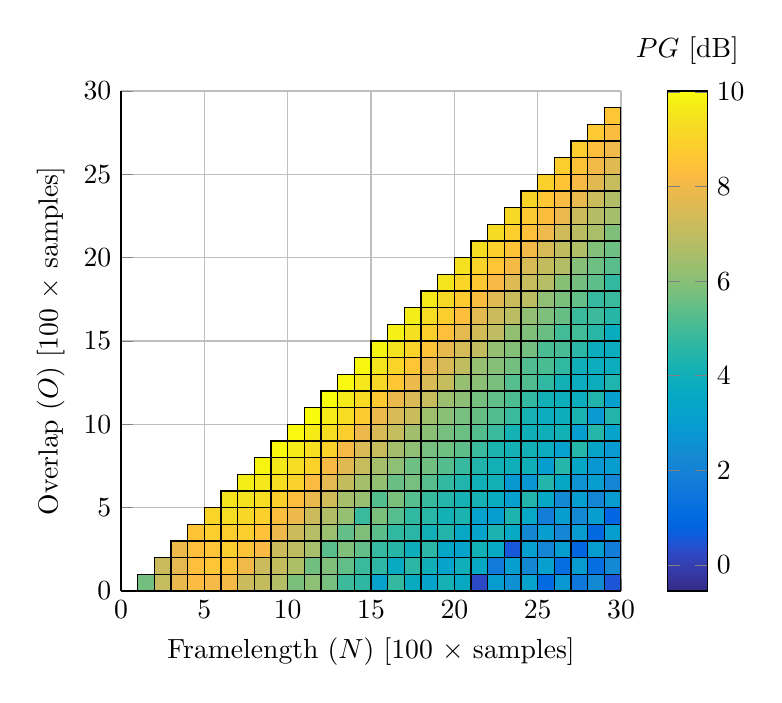
\begin{tikzpicture}


\begin{axis}[%
width=2.5in,
height=2.5in,
scale only axis,
point meta min=-0.551769511455843,
point meta max=10.0207598959184,
unbounded coords=jump,
xmin=0,
xmax=3000,
xlabel={Framelength ($N$) [100 $\times$ samples]},
xmajorgrids,
ymin=0,
ymax=3000,
ytick={0,500,...,3000},
yticklabels={0,5,...,30},
xtick={0,500,...,3000},
xticklabels={0,5,...,30},
ylabel={Overlap ($O$) [100 $\times$ samples]},
ymajorgrids,
axis background/.style={fill=white},
axis x line*=bottom,
axis y line*=left,
colormap={mymap}{[1pt] rgb(0pt)=(0.2081,0.1663,0.5292); rgb(1pt)=(0.211624,0.189781,0.577676); rgb(2pt)=(0.212252,0.213771,0.626971); rgb(3pt)=(0.2081,0.2386,0.677086); rgb(4pt)=(0.195905,0.264457,0.7279); rgb(5pt)=(0.170729,0.291938,0.779248); rgb(6pt)=(0.125271,0.324243,0.830271); rgb(7pt)=(0.0591333,0.359833,0.868333); rgb(8pt)=(0.0116952,0.38751,0.881957); rgb(9pt)=(0.00595714,0.408614,0.882843); rgb(10pt)=(0.0165143,0.4266,0.878633); rgb(11pt)=(0.0328524,0.443043,0.871957); rgb(12pt)=(0.0498143,0.458571,0.864057); rgb(13pt)=(0.0629333,0.47369,0.855438); rgb(14pt)=(0.0722667,0.488667,0.8467); rgb(15pt)=(0.0779429,0.503986,0.838371); rgb(16pt)=(0.0793476,0.520024,0.831181); rgb(17pt)=(0.0749429,0.537543,0.826271); rgb(18pt)=(0.0640571,0.556986,0.823957); rgb(19pt)=(0.0487714,0.577224,0.822829); rgb(20pt)=(0.0343429,0.596581,0.819852); rgb(21pt)=(0.0265,0.6137,0.8135); rgb(22pt)=(0.0238905,0.628662,0.803762); rgb(23pt)=(0.0230905,0.641786,0.791267); rgb(24pt)=(0.0227714,0.653486,0.776757); rgb(25pt)=(0.0266619,0.664195,0.760719); rgb(26pt)=(0.0383714,0.674271,0.743552); rgb(27pt)=(0.0589714,0.683757,0.725386); rgb(28pt)=(0.0843,0.692833,0.706167); rgb(29pt)=(0.113295,0.7015,0.685857); rgb(30pt)=(0.145271,0.709757,0.664629); rgb(31pt)=(0.180133,0.717657,0.642433); rgb(32pt)=(0.217829,0.725043,0.619262); rgb(33pt)=(0.258643,0.731714,0.595429); rgb(34pt)=(0.302171,0.737605,0.571186); rgb(35pt)=(0.348167,0.742433,0.547267); rgb(36pt)=(0.395257,0.7459,0.524443); rgb(37pt)=(0.44201,0.748081,0.503314); rgb(38pt)=(0.487124,0.749062,0.483976); rgb(39pt)=(0.530029,0.749114,0.466114); rgb(40pt)=(0.570857,0.748519,0.44939); rgb(41pt)=(0.609852,0.747314,0.433686); rgb(42pt)=(0.6473,0.7456,0.4188); rgb(43pt)=(0.683419,0.743476,0.404433); rgb(44pt)=(0.71841,0.741133,0.390476); rgb(45pt)=(0.752486,0.7384,0.376814); rgb(46pt)=(0.785843,0.735567,0.363271); rgb(47pt)=(0.818505,0.732733,0.34979); rgb(48pt)=(0.850657,0.7299,0.336029); rgb(49pt)=(0.882433,0.727433,0.3217); rgb(50pt)=(0.913933,0.725786,0.306276); rgb(51pt)=(0.944957,0.726114,0.288643); rgb(52pt)=(0.973895,0.731395,0.266648); rgb(53pt)=(0.993771,0.745457,0.240348); rgb(54pt)=(0.999043,0.765314,0.216414); rgb(55pt)=(0.995533,0.786057,0.196652); rgb(56pt)=(0.988,0.8066,0.179367); rgb(57pt)=(0.978857,0.827143,0.163314); rgb(58pt)=(0.9697,0.848138,0.147452); rgb(59pt)=(0.962586,0.870514,0.1309); rgb(60pt)=(0.958871,0.8949,0.113243); rgb(61pt)=(0.959824,0.921833,0.0948381); rgb(62pt)=(0.9661,0.951443,0.0755333); rgb(63pt)=(0.9763,0.9831,0.0538)},
colorbar,
colorbar style={title=$PG$ [dB]}
]%ylabel={PG}

\addplot[%
surf,
opacity = ceil(\pgfplotspointmetatransformed),
shader=flat corner,draw=black,colormap={mymap}{[1pt] rgb(0pt)=(0.2081,0.1663,0.5292); rgb(1pt)=(0.211624,0.189781,0.577676); rgb(2pt)=(0.212252,0.213771,0.626971); rgb(3pt)=(0.2081,0.2386,0.677086); rgb(4pt)=(0.195905,0.264457,0.7279); rgb(5pt)=(0.170729,0.291938,0.779248); rgb(6pt)=(0.125271,0.324243,0.830271); rgb(7pt)=(0.0591333,0.359833,0.868333); rgb(8pt)=(0.0116952,0.38751,0.881957); rgb(9pt)=(0.00595714,0.408614,0.882843); rgb(10pt)=(0.0165143,0.4266,0.878633); rgb(11pt)=(0.0328524,0.443043,0.871957); rgb(12pt)=(0.0498143,0.458571,0.864057); rgb(13pt)=(0.0629333,0.47369,0.855438); rgb(14pt)=(0.0722667,0.488667,0.8467); rgb(15pt)=(0.0779429,0.503986,0.838371); rgb(16pt)=(0.0793476,0.520024,0.831181); rgb(17pt)=(0.0749429,0.537543,0.826271); rgb(18pt)=(0.0640571,0.556986,0.823957); rgb(19pt)=(0.0487714,0.577224,0.822829); rgb(20pt)=(0.0343429,0.596581,0.819852); rgb(21pt)=(0.0265,0.6137,0.8135); rgb(22pt)=(0.0238905,0.628662,0.803762); rgb(23pt)=(0.0230905,0.641786,0.791267); rgb(24pt)=(0.0227714,0.653486,0.776757); rgb(25pt)=(0.0266619,0.664195,0.760719); rgb(26pt)=(0.0383714,0.674271,0.743552); rgb(27pt)=(0.0589714,0.683757,0.725386); rgb(28pt)=(0.0843,0.692833,0.706167); rgb(29pt)=(0.113295,0.7015,0.685857); rgb(30pt)=(0.145271,0.709757,0.664629); rgb(31pt)=(0.180133,0.717657,0.642433); rgb(32pt)=(0.217829,0.725043,0.619262); rgb(33pt)=(0.258643,0.731714,0.595429); rgb(34pt)=(0.302171,0.737605,0.571186); rgb(35pt)=(0.348167,0.742433,0.547267); rgb(36pt)=(0.395257,0.7459,0.524443); rgb(37pt)=(0.44201,0.748081,0.503314); rgb(38pt)=(0.487124,0.749062,0.483976); rgb(39pt)=(0.530029,0.749114,0.466114); rgb(40pt)=(0.570857,0.748519,0.44939); rgb(41pt)=(0.609852,0.747314,0.433686); rgb(42pt)=(0.6473,0.7456,0.4188); rgb(43pt)=(0.683419,0.743476,0.404433); rgb(44pt)=(0.71841,0.741133,0.390476); rgb(45pt)=(0.752486,0.7384,0.376814); rgb(46pt)=(0.785843,0.735567,0.363271); rgb(47pt)=(0.818505,0.732733,0.34979); rgb(48pt)=(0.850657,0.7299,0.336029); rgb(49pt)=(0.882433,0.727433,0.3217); rgb(50pt)=(0.913933,0.725786,0.306276); rgb(51pt)=(0.944957,0.726114,0.288643); rgb(52pt)=(0.973895,0.731395,0.266648); rgb(53pt)=(0.993771,0.745457,0.240348); rgb(54pt)=(0.999043,0.765314,0.216414); rgb(55pt)=(0.995533,0.786057,0.196652); rgb(56pt)=(0.988,0.8066,0.179367); rgb(57pt)=(0.978857,0.827143,0.163314); rgb(58pt)=(0.9697,0.848138,0.147452); rgb(59pt)=(0.962586,0.870514,0.1309); rgb(60pt)=(0.958871,0.8949,0.113243); rgb(61pt)=(0.959824,0.921833,0.0948381); rgb(62pt)=(0.9661,0.951443,0.0755333); rgb(63pt)=(0.9763,0.9831,0.0538)},mesh/rows=30]
table[row sep=crcr, point meta=\thisrow{c}] {%
%
x	y	c\\
100	0	5.6827458135075\\
100	100	nan\\
100	200	nan\\
100	300	nan\\
100	400	nan\\
100	500	nan\\
100	600	nan\\
100	700	nan\\
100	800	nan\\
100	900	nan\\
100	1000	nan\\
100	1100	nan\\
100	1200	nan\\
100	1300	nan\\
100	1400	nan\\
100	1500	nan\\
100	1600	nan\\
100	1700	nan\\
100	1800	nan\\
100	1900	nan\\
100	2000	nan\\
100	2100	nan\\
100	2200	nan\\
100	2300	nan\\
100	2400	nan\\
100	2500	nan\\
100	2600	nan\\
100	2700	nan\\
100	2800	nan\\
100	2900	nan\\
200	0	7.0790317182078\\
200	100	7.18389489543295\\
200	200	nan\\
200	300	nan\\
200	400	nan\\
200	500	nan\\
200	600	nan\\
200	700	nan\\
200	800	nan\\
200	900	nan\\
200	1000	nan\\
200	1100	nan\\
200	1200	nan\\
200	1300	nan\\
200	1400	nan\\
200	1500	nan\\
200	1600	nan\\
200	1700	nan\\
200	1800	nan\\
200	1900	nan\\
200	2000	nan\\
200	2100	nan\\
200	2200	nan\\
200	2300	nan\\
200	2400	nan\\
200	2500	nan\\
200	2600	nan\\
200	2700	nan\\
200	2800	nan\\
200	2900	nan\\
300	0	7.8278797182668\\
300	100	7.75061670667307\\
300	200	7.94964232573768\\
300	300	nan\\
300	400	nan\\
300	500	nan\\
300	600	nan\\
300	700	nan\\
300	800	nan\\
300	900	nan\\
300	1000	nan\\
300	1100	nan\\
300	1200	nan\\
300	1300	nan\\
300	1400	nan\\
300	1500	nan\\
300	1600	nan\\
300	1700	nan\\
300	1800	nan\\
300	1900	nan\\
300	2000	nan\\
300	2100	nan\\
300	2200	nan\\
300	2300	nan\\
300	2400	nan\\
300	2500	nan\\
300	2600	nan\\
300	2700	nan\\
300	2800	nan\\
300	2900	nan\\
400	0	8.25982045157361\\
400	100	8.37365829237133\\
400	200	8.38994845512447\\
400	300	8.53395155897113\\
400	400	nan\\
400	500	nan\\
400	600	nan\\
400	700	nan\\
400	800	nan\\
400	900	nan\\
400	1000	nan\\
400	1100	nan\\
400	1200	nan\\
400	1300	nan\\
400	1400	nan\\
400	1500	nan\\
400	1600	nan\\
400	1700	nan\\
400	1800	nan\\
400	1900	nan\\
400	2000	nan\\
400	2100	nan\\
400	2200	nan\\
400	2300	nan\\
400	2400	nan\\
400	2500	nan\\
400	2600	nan\\
400	2700	nan\\
400	2800	nan\\
400	2900	nan\\
500	0	8.09522110947221\\
500	100	8.58404936019439\\
500	200	8.52476852167647\\
500	300	8.85395289600773\\
500	400	9.03400135477561\\
500	500	nan\\
500	600	nan\\
500	700	nan\\
500	800	nan\\
500	900	nan\\
500	1000	nan\\
500	1100	nan\\
500	1200	nan\\
500	1300	nan\\
500	1400	nan\\
500	1500	nan\\
500	1600	nan\\
500	1700	nan\\
500	1800	nan\\
500	1900	nan\\
500	2000	nan\\
500	2100	nan\\
500	2200	nan\\
500	2300	nan\\
500	2400	nan\\
500	2500	nan\\
500	2600	nan\\
500	2700	nan\\
500	2800	nan\\
500	2900	nan\\
600	0	8.05650724153339\\
600	100	8.54693570913705\\
600	200	8.8377683265956\\
600	300	8.82559971223848\\
600	400	9.28658312212634\\
600	500	9.52161535433559\\
600	600	nan\\
600	700	nan\\
600	800	nan\\
600	900	nan\\
600	1000	nan\\
600	1100	nan\\
600	1200	nan\\
600	1300	nan\\
600	1400	nan\\
600	1500	nan\\
600	1600	nan\\
600	1700	nan\\
600	1800	nan\\
600	1900	nan\\
600	2000	nan\\
600	2100	nan\\
600	2200	nan\\
600	2300	nan\\
600	2400	nan\\
600	2500	nan\\
600	2600	nan\\
600	2700	nan\\
600	2800	nan\\
600	2900	nan\\
700	0	7.20736652003549\\
700	100	8.01860060821804\\
700	200	8.5092217869215\\
700	300	8.85498614721321\\
700	400	9.13100370114176\\
700	500	9.43150883603405\\
700	600	9.74782220562509\\
700	700	nan\\
700	800	nan\\
700	900	nan\\
700	1000	nan\\
700	1100	nan\\
700	1200	nan\\
700	1300	nan\\
700	1400	nan\\
700	1500	nan\\
700	1600	nan\\
700	1700	nan\\
700	1800	nan\\
700	1900	nan\\
700	2000	nan\\
700	2100	nan\\
700	2200	nan\\
700	2300	nan\\
700	2400	nan\\
700	2500	nan\\
700	2600	nan\\
700	2700	nan\\
700	2800	nan\\
700	2900	nan\\
800	0	7.06129617908756\\
800	100	7.21625389795336\\
800	200	8.17024678080842\\
800	300	8.4506398874489\\
800	400	8.92543148972206\\
800	500	9.31059383665309\\
800	600	9.57358732259701\\
800	700	9.88474425342921\\
800	800	nan\\
800	900	nan\\
800	1000	nan\\
800	1100	nan\\
800	1200	nan\\
800	1300	nan\\
800	1400	nan\\
800	1500	nan\\
800	1600	nan\\
800	1700	nan\\
800	1800	nan\\
800	1900	nan\\
800	2000	nan\\
800	2100	nan\\
800	2200	nan\\
800	2300	nan\\
800	2400	nan\\
800	2500	nan\\
800	2600	nan\\
800	2700	nan\\
800	2800	nan\\
800	2900	nan\\
900	0	6.7603240209297\\
900	100	7.07027516643772\\
900	200	7.21503157848168\\
900	300	7.91680228410601\\
900	400	8.33413384154289\\
900	500	8.91700110520262\\
900	600	9.33441266257382\\
900	700	9.61050000584357\\
900	800	9.96602273571317\\
900	900	nan\\
900	1000	nan\\
900	1100	nan\\
900	1200	nan\\
900	1300	nan\\
900	1400	nan\\
900	1500	nan\\
900	1600	nan\\
900	1700	nan\\
900	1800	nan\\
900	1900	nan\\
900	2000	nan\\
900	2100	nan\\
900	2200	nan\\
900	2300	nan\\
900	2400	nan\\
900	2500	nan\\
900	2600	nan\\
900	2700	nan\\
900	2800	nan\\
900	2900	nan\\
1000	0	5.79141266758575\\
1000	100	6.6583846543796\\
1000	200	6.96560213501504\\
1000	300	7.24068731658401\\
1000	400	7.9395591224285\\
1000	500	8.31867811054653\\
1000	600	8.9754932003346\\
1000	700	9.34845065231673\\
1000	800	9.67344129050852\\
1000	900	9.99470564606262\\
1000	1000	nan\\
1000	1100	nan\\
1000	1200	nan\\
1000	1300	nan\\
1000	1400	nan\\
1000	1500	nan\\
1000	1600	nan\\
1000	1700	nan\\
1000	1800	nan\\
1000	1900	nan\\
1000	2000	nan\\
1000	2100	nan\\
1000	2200	nan\\
1000	2300	nan\\
1000	2400	nan\\
1000	2500	nan\\
1000	2600	nan\\
1000	2700	nan\\
1000	2800	nan\\
1000	2900	nan\\
1100	0	6.08510006030311\\
1100	100	5.66131684642677\\
1100	200	6.52494101151453\\
1100	300	6.8154749961067\\
1100	400	7.2221683246724\\
1100	500	7.85272239575603\\
1100	600	8.25834444268623\\
1100	700	8.98246828788382\\
1100	800	9.38384280669374\\
1100	900	9.67888280713376\\
1100	1000	10.0207598959184\\
1100	1100	nan\\
1100	1200	nan\\
1100	1300	nan\\
1100	1400	nan\\
1100	1500	nan\\
1100	1600	nan\\
1100	1700	nan\\
1100	1800	nan\\
1100	1900	nan\\
1100	2000	nan\\
1100	2100	nan\\
1100	2200	nan\\
1100	2300	nan\\
1100	2400	nan\\
1100	2500	nan\\
1100	2600	nan\\
1100	2700	nan\\
1100	2800	nan\\
1100	2900	nan\\
1200	0	5.75236385929885\\
1200	100	5.8893978793085\\
1200	200	5.3233876826882\\
1200	300	6.30245671838949\\
1200	400	6.70416183583482\\
1200	500	7.29231639499116\\
1200	600	7.73083236703484\\
1200	700	8.13278866080154\\
1200	800	8.95016901139914\\
1200	900	9.3575654964583\\
1200	1000	9.69962351631871\\
1200	1100	10.018452727616\\
1200	1200	nan\\
1200	1300	nan\\
1200	1400	nan\\
1200	1500	nan\\
1200	1600	nan\\
1200	1700	nan\\
1200	1800	nan\\
1200	1900	nan\\
1200	2000	nan\\
1200	2100	nan\\
1200	2200	nan\\
1200	2300	nan\\
1200	2400	nan\\
1200	2500	nan\\
1200	2600	nan\\
1200	2700	nan\\
1200	2800	nan\\
1200	2900	nan\\
1300	0	4.8910628019805\\
1300	100	5.45072016874233\\
1300	200	5.86850066777867\\
1300	300	5.4597166268533\\
1300	400	6.21490882072339\\
1300	500	6.48849191466192\\
1300	600	7.05573401013256\\
1300	700	7.66870480877405\\
1300	800	8.12020714201073\\
1300	900	8.84241536316059\\
1300	1000	9.32521343768448\\
1300	1100	9.66682615033229\\
1300	1200	9.99393859933556\\
1300	1300	nan\\
1300	1400	nan\\
1300	1500	nan\\
1300	1600	nan\\
1300	1700	nan\\
1300	1800	nan\\
1300	1900	nan\\
1300	2000	nan\\
1300	2100	nan\\
1300	2200	nan\\
1300	2300	nan\\
1300	2400	nan\\
1300	2500	nan\\
1300	2600	nan\\
1300	2700	nan\\
1300	2800	nan\\
1300	2900	nan\\
1400	0	4.68328180207416\\
1400	100	4.87031890586883\\
1400	200	5.46124064783872\\
1400	300	5.87957713868692\\
1400	400	4.86401495955569\\
1400	500	6.26391766665361\\
1400	600	6.48566475687751\\
1400	700	7.13851035956643\\
1400	800	7.50027034876972\\
1400	900	7.94746340189027\\
1400	1000	8.77453134934714\\
1400	1100	9.23762319980819\\
1400	1200	9.58536439829166\\
1400	1300	9.93647418346277\\
1400	1400	nan\\
1400	1500	nan\\
1400	1600	nan\\
1400	1700	nan\\
1400	1800	nan\\
1400	1900	nan\\
1400	2000	nan\\
1400	2100	nan\\
1400	2200	nan\\
1400	2300	nan\\
1400	2400	nan\\
1400	2500	nan\\
1400	2600	nan\\
1400	2700	nan\\
1400	2800	nan\\
1400	2900	nan\\
1500	0	3.24765243794076\\
1500	100	4.65481232593174\\
1500	200	4.79830988957897\\
1500	300	5.35751567095906\\
1500	400	5.79287838471904\\
1500	500	5.25522140259071\\
1500	600	6.17072553135157\\
1500	700	6.48214041903959\\
1500	800	7.1345332299744\\
1500	900	7.48068047659614\\
1500	1000	7.89377405226484\\
1500	1100	8.70610504087698\\
1500	1200	9.16324372984275\\
1500	1300	9.52474035946379\\
1500	1400	9.86030813520319\\
1500	1500	nan\\
1500	1600	nan\\
1500	1700	nan\\
1500	1800	nan\\
1500	1900	nan\\
1500	2000	nan\\
1500	2100	nan\\
1500	2200	nan\\
1500	2300	nan\\
1500	2400	nan\\
1500	2500	nan\\
1500	2600	nan\\
1500	2700	nan\\
1500	2800	nan\\
1500	2900	nan\\
1600	0	4.75276003383697\\
1600	100	3.67495640572055\\
1600	200	4.52251715002299\\
1600	300	4.70771251796696\\
1600	400	5.26201893473007\\
1600	500	5.81200015855313\\
1600	600	5.54198269350814\\
1600	700	6.09112217072302\\
1600	800	6.43437379918348\\
1600	900	7.09943797512656\\
1600	1000	7.48241897845622\\
1600	1100	7.90693168041642\\
1600	1200	8.6380368658202\\
1600	1300	9.0916878406797\\
1600	1400	9.45586978035725\\
1600	1500	9.79114079162636\\
1600	1600	nan\\
1600	1700	nan\\
1600	1800	nan\\
1600	1900	nan\\
1600	2000	nan\\
1600	2100	nan\\
1600	2200	nan\\
1600	2300	nan\\
1600	2400	nan\\
1600	2500	nan\\
1600	2600	nan\\
1600	2700	nan\\
1600	2800	nan\\
1600	2900	nan\\
1700	0	3.71748664243527\\
1700	100	4.60591980476924\\
1700	200	3.91362630267876\\
1700	300	4.55847242510564\\
1700	400	4.70161157949911\\
1700	500	5.26688872672145\\
1700	600	5.74077415219596\\
1700	700	5.60918413969161\\
1700	800	6.12512258839059\\
1700	900	6.40152380276071\\
1700	1000	7.16577614393491\\
1700	1100	7.4954835376692\\
1700	1200	7.90408510720934\\
1700	1300	8.57357709454054\\
1700	1400	9.0277543415418\\
1700	1500	9.3764265164728\\
1700	1600	9.7243052974142\\
1700	1700	nan\\
1700	1800	nan\\
1700	1900	nan\\
1700	2000	nan\\
1700	2100	nan\\
1700	2200	nan\\
1700	2300	nan\\
1700	2400	nan\\
1700	2500	nan\\
1700	2600	nan\\
1700	2700	nan\\
1700	2800	nan\\
1700	2900	nan\\
1800	0	3.3177087556264\\
1800	100	4.01520154764494\\
1800	200	4.58897692120239\\
1800	300	4.05120880760072\\
1800	400	4.53307279512351\\
1800	500	4.80647025338146\\
1800	600	5.30764576164913\\
1800	700	5.66202006578872\\
1800	800	5.75312164595155\\
1800	900	6.04395256930141\\
1800	1000	6.3700405132766\\
1800	1100	7.14316992342896\\
1800	1200	7.48470310198768\\
1800	1300	7.87037714378024\\
1800	1400	8.48717243248572\\
1800	1500	8.92938209706209\\
1800	1600	9.3014704008889\\
1800	1700	9.64275886586559\\
1800	1800	nan\\
1800	1900	nan\\
1800	2000	nan\\
1800	2100	nan\\
1800	2200	nan\\
1800	2300	nan\\
1800	2400	nan\\
1800	2500	nan\\
1800	2600	nan\\
1800	2700	nan\\
1800	2800	nan\\
1800	2900	nan\\
1900	0	4.16438107268957\\
1900	100	3.30621453732177\\
1900	200	3.45177011062336\\
1900	300	4.41976545924296\\
1900	400	4.07826463673203\\
1900	500	4.47250181773447\\
1900	600	4.74401157157616\\
1900	700	5.27110068830706\\
1900	800	5.6301314654757\\
1900	900	5.74823980250472\\
1900	1000	6.03395598979113\\
1900	1100	6.3316791328726\\
1900	1200	7.11053211593739\\
1900	1300	7.45923534882344\\
1900	1400	7.81374082935247\\
1900	1500	8.40334989731675\\
1900	1600	8.81911874169977\\
1900	1700	9.19800880789435\\
1900	1800	9.54583520361966\\
1900	1900	nan\\
1900	2000	nan\\
1900	2100	nan\\
1900	2200	nan\\
1900	2300	nan\\
1900	2400	nan\\
1900	2500	nan\\
1900	2600	nan\\
1900	2700	nan\\
1900	2800	nan\\
1900	2900	nan\\
2000	0	3.63837130417713\\
2000	100	3.96838494244702\\
2000	200	3.28360542391229\\
2000	300	3.55278143786063\\
2000	400	4.26805123856089\\
2000	500	4.15389920807166\\
2000	600	4.39329679744196\\
2000	700	4.78828316129288\\
2000	800	5.37993737198608\\
2000	900	5.58147465390246\\
2000	1000	5.7286955025126\\
2000	1100	6.07285315548354\\
2000	1200	6.23857857671884\\
2000	1300	7.01013622331059\\
2000	1400	7.40631428562525\\
2000	1500	7.74343597295201\\
2000	1600	8.32757229622458\\
2000	1700	8.74188942454939\\
2000	1800	9.09209523315045\\
2000	1900	9.44134118935649\\
2000	2000	nan\\
2000	2100	nan\\
2000	2200	nan\\
2000	2300	nan\\
2000	2400	nan\\
2000	2500	nan\\
2000	2600	nan\\
2000	2700	nan\\
2000	2800	nan\\
2000	2900	nan\\
2100	0	0.264623542453294\\
2100	100	3.63488656288565\\
2100	200	4.08913120930422\\
2100	300	3.28220109142383\\
2100	400	3.18039510652367\\
2100	500	4.19474057968373\\
2100	600	4.0275612369305\\
2100	700	4.39427002201494\\
2100	800	4.86473111214704\\
2100	900	5.25381195203792\\
2100	1000	5.52645898428144\\
2100	1100	5.71270454803943\\
2100	1200	6.05580569501984\\
2100	1300	6.23707654312965\\
2100	1400	7.00000513992408\\
2100	1500	7.3381894461935\\
2100	1600	7.70510502361266\\
2100	1700	8.27878784954097\\
2100	1800	8.66979451640054\\
2100	1900	9.0155911617751\\
2100	2000	9.34506416881835\\
2100	2100	nan\\
2100	2200	nan\\
2100	2300	nan\\
2100	2400	nan\\
2100	2500	nan\\
2100	2600	nan\\
2100	2700	nan\\
2100	2800	nan\\
2100	2900	nan\\
2200	0	2.95170309874089\\
2200	100	1.73360893357364\\
2200	200	3.61323080676111\\
2200	300	4.28061341062458\\
2200	400	3.02458697343151\\
2200	500	3.75811713713825\\
2200	600	4.06218778116715\\
2200	700	4.05610248843421\\
2200	800	4.30007538322245\\
2200	900	4.85697872751457\\
2200	1000	5.22977855686604\\
2200	1100	5.42728488717261\\
2200	1200	5.7742976825497\\
2200	1300	5.9578809065615\\
2200	1400	6.20369481654021\\
2200	1500	6.97748546317166\\
2200	1600	7.25905430947499\\
2200	1700	7.63071051415358\\
2200	1800	8.17187520251639\\
2200	1900	8.56846748612261\\
2200	2000	8.92936194092831\\
2200	2100	9.25326090597395\\
2200	2200	nan\\
2200	2300	nan\\
2200	2400	nan\\
2200	2500	nan\\
2200	2600	nan\\
2200	2700	nan\\
2200	2800	nan\\
2200	2900	nan\\
2300	0	2.53293217519118\\
2300	100	3.00938026182184\\
2300	200	0.551769511455843\\
2300	300	3.60726664380354\\
2300	400	4.36229780994093\\
2300	500	3.08643225262487\\
2300	600	2.82564622459287\\
2300	700	3.98306729613317\\
2300	800	4.11490314132238\\
2300	900	4.13618785976634\\
2300	1000	4.86317380717345\\
2300	1100	5.16517700158233\\
2300	1200	5.26664183435126\\
2300	1300	5.69684803139814\\
2300	1400	5.95135216558113\\
2300	1500	6.16719875147937\\
2300	1600	6.89154945837155\\
2300	1700	7.18393537254356\\
2300	1800	7.60032386475286\\
2300	1900	8.1060139824226\\
2300	2000	8.49168618698787\\
2300	2100	8.84145695288964\\
2300	2200	9.16963549024874\\
2300	2300	nan\\
2300	2400	nan\\
2300	2500	nan\\
2300	2600	nan\\
2300	2700	nan\\
2300	2800	nan\\
2300	2900	nan\\
2400	0	3.23692740006642\\
2400	100	2.2228524336536\\
2400	200	3.08472299555247\\
2400	300	2.2240377386973\\
2400	400	3.53887086816519\\
2400	500	4.42615653537038\\
2400	600	2.75840359129067\\
2400	700	4.0107386280573\\
2400	800	4.05214769333313\\
2400	900	4.00914531419853\\
2400	1000	4.17937149969251\\
2400	1100	4.74117848303689\\
2400	1200	5.2085286363726\\
2400	1300	5.19304330014419\\
2400	1400	5.69847355162021\\
2400	1500	5.87188705075393\\
2400	1600	6.15489171474828\\
2400	1700	6.89765995399639\\
2400	1800	7.11879031436815\\
2400	1900	7.49046026449902\\
2400	2000	8.04502341053814\\
2400	2100	8.40465258616035\\
2400	2200	8.73328129071907\\
2400	2300	9.06128194950849\\
2400	2400	nan\\
2400	2500	nan\\
2400	2600	nan\\
2400	2700	nan\\
2400	2800	nan\\
2400	2900	nan\\
2500	0	1.05000257678802\\
2500	100	3.09955807465487\\
2500	200	2.13019145244393\\
2500	300	2.98129659738565\\
2500	400	1.80823551110839\\
2500	500	3.44295461285468\\
2500	600	4.45023506033534\\
2500	700	3.03486862485067\\
2500	800	3.799754032993\\
2500	900	3.97648541270297\\
2500	1000	3.83352254491892\\
2500	1100	4.04591105923088\\
2500	1200	4.69567516678935\\
2500	1300	5.11099504335296\\
2500	1400	5.09859465247581\\
2500	1500	5.57858218898721\\
2500	1600	5.8569467833986\\
2500	1700	6.10341874446816\\
2500	1800	6.81391868519097\\
2500	1900	7.03573319906174\\
2500	2000	7.42018466644079\\
2500	2100	7.9589647003702\\
2500	2200	8.29921705504155\\
2500	2300	8.63637971004693\\
2500	2400	8.96380635737141\\
2500	2500	nan\\
2500	2600	nan\\
2500	2700	nan\\
2500	2800	nan\\
2500	2900	nan\\
2600	0	2.80208415075651\\
2600	100	1.17194843956108\\
2600	200	2.96109260453396\\
2600	300	2.19270843592341\\
2600	400	3.0115728867441\\
2600	500	2.28393968299924\\
2600	600	3.47369768467374\\
2600	700	4.50853743880052\\
2600	800	3.15812371844604\\
2600	900	4.07856863803736\\
2600	1000	3.91468626002954\\
2600	1100	3.89808210094217\\
2600	1200	4.04567753651072\\
2600	1300	4.70566985097843\\
2600	1400	5.07194378908158\\
2600	1500	4.99752267777982\\
2600	1600	5.52550384847648\\
2600	1700	5.79174211203976\\
2600	1800	6.00046246850643\\
2600	1900	6.74511848933576\\
2600	2000	6.98699179435392\\
2600	2100	7.31013917497011\\
2600	2200	7.87653800818457\\
2600	2300	8.22494050640918\\
2600	2400	8.54322091765009\\
2600	2500	8.85820789226427\\
2600	2600	nan\\
2600	2700	nan\\
2600	2800	nan\\
2600	2900	nan\\
2700	0	1.58184394833386\\
2700	100	2.92525400331244\\
2700	200	0.887359676794604\\
2700	300	2.93101822389555\\
2700	400	2.30024404624266\\
2700	500	3.00032580576816\\
2700	600	2.58705024710389\\
2700	700	3.44496986930798\\
2700	800	4.4916042025927\\
2700	900	2.98522379998911\\
2700	1000	4.25749977657229\\
2700	1100	3.87067312264047\\
2700	1200	3.83784894949447\\
2700	1300	3.98929857887126\\
2700	1400	4.59197088590304\\
2700	1500	4.99312405800586\\
2700	1600	4.86180118194934\\
2700	1700	5.46261986535732\\
2700	1800	5.70973165052257\\
2700	1900	5.97276788996415\\
2700	2000	6.67403857872095\\
2700	2100	6.91286174850295\\
2700	2200	7.25280658811363\\
2700	2300	7.81626379934614\\
2700	2400	8.13648239969618\\
2700	2500	8.46913649633422\\
2700	2600	8.78457026475621\\
2700	2700	nan\\
2700	2800	nan\\
2700	2900	nan\\
2800	0	2.2987560540242\\
2800	100	1.19896433152671\\
2800	200	2.95163573066064\\
2800	300	0.973202079270705\\
2800	400	2.97370455963156\\
2800	500	2.12856324963795\\
2800	600	2.98222869928969\\
2800	700	2.77033362268512\\
2800	800	3.38784440474213\\
2800	900	4.50283031414694\\
2800	1000	2.86687295264398\\
2800	1100	4.3797702935594\\
2800	1200	3.86077604223459\\
2800	1300	3.88445747215116\\
2800	1400	3.88641891122799\\
2800	1500	4.54099461834347\\
2800	1600	4.89171252973565\\
2800	1700	4.80102017502878\\
2800	1800	5.38055416094404\\
2800	1900	5.62096395390293\\
2800	2000	5.9064550594499\\
2800	2100	6.57396144817971\\
2800	2200	6.77884258803287\\
2800	2300	7.20159987892983\\
2800	2400	7.70137646156138\\
2800	2500	8.02001565102648\\
2800	2600	8.3537017651593\\
2800	2700	8.6861911739627\\
2800	2800	nan\\
2800	2900	nan\\
2900	0	0.49312967237007\\
2900	100	2.25840014462245\\
2900	200	1.80380427347787\\
2900	300	3.03746280090745\\
2900	400	0.845717353642782\\
2900	500	2.91980222011896\\
2900	600	2.20120210963457\\
2900	700	2.99077861803715\\
2900	800	2.87641657842737\\
2900	900	3.26134076790394\\
2900	1000	4.42889490862495\\
2900	1100	3.07565824698724\\
2900	1200	4.36835391429797\\
2900	1300	3.8835622884345\\
2900	1400	3.84533451378335\\
2900	1500	3.78342493811934\\
2900	1600	4.5195926660129\\
2900	1700	4.84979739867748\\
2900	1800	4.72342685477777\\
2900	1900	5.32512315595608\\
2900	2000	5.60997138907586\\
2900	2100	5.87473951276466\\
2900	2200	6.48270953309765\\
2900	2300	6.71059287812374\\
2900	2400	7.1263819393935\\
2900	2500	7.63768597628047\\
2900	2600	7.95785638792816\\
2900	2700	8.27184455059282\\
2900	2800	8.58887864737359\\
2900	2900	nan\\
3000	0	-0.084166652386565\\
3000	100	0.658799202686103\\
3000	200	2.4286786445431\\
3000	300	2.00173215444182\\
3000	400	3.04605438638216\\
3000	500	0.804121831033953\\
3000	600	2.80060747061573\\
3000	700	2.10723369617921\\
3000	800	3.00606491677149\\
3000	900	2.9921027849289\\
3000	1000	3.2003941437714\\
3000	1100	4.47914328347861\\
3000	1200	3.09026222985996\\
3000	1300	4.40877799382241\\
3000	1400	3.86783693309201\\
3000	1500	3.82141825431614\\
3000	1600	3.75968653309083\\
3000	1700	4.42136187911435\\
3000	1800	4.73062760871956\\
3000	1900	4.65092537646692\\
3000	2000	5.26464935536502\\
3000	2100	5.53276290699877\\
3000	2200	5.79426518264794\\
3000	2300	6.43034113528171\\
3000	2400	6.61621727344431\\
3000	2500	6.98815251985862\\
3000	2600	7.51974760550906\\
3000	2700	7.84037752158828\\
3000	2800	8.1530922590658\\
3000	2900	8.49883156713133\\
};
\end{axis}
\end{tikzpicture}%}
	\end{column}
\end{columns}
\end{frame}

\begin{frame}{Simulation Results}{Optimal parameters}		
\begin{columns}
	\begin{column}{0.4\textwidth}
	\begin{itemize}
		\item Prediction order P = 3
		\item Optimal parameters
		\begin{itemize}
			\item Framelength N = 300
			\item Overlap O = 250
		\end{itemize}
		\item Prediction Gain PG = 8.5 dB
	\end{itemize}
	\end{column}
	\begin{column}{0.6\textwidth} 
		\resizebox{0.9\columnwidth}{!}{		
			% This file was created by matlab2tikz.
%
%The latest updates can be retrieved from
%  http://www.mathworks.com/matlabcentral/fileexchange/22022-matlab2tikz-matlab2tikz
%where you can also make suggestions and rate matlab2tikz.
%
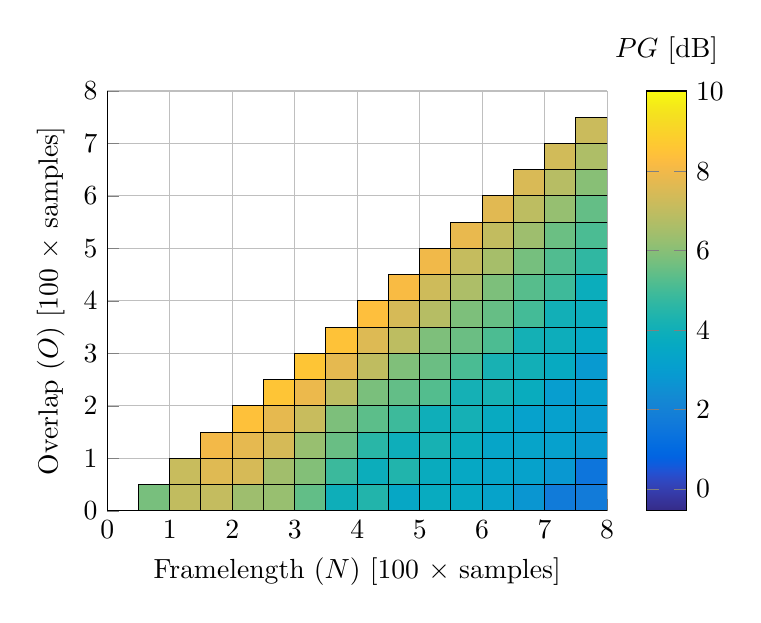
\begin{tikzpicture}

%\begin{axis}[%
%width=3.891in,
%height=3.566in,
%at={(0.653in,0.481in)},
%scale only axis,
%point meta min=0.606438537667243,
%point meta max=8.58051607966271,
%unbounded coords=jump,
%xmin=0,
%xmax=800,
%xlabel={Framelength (N) [samples]},
%xmajorgrids,
%ymin=0,
%ymax=800,
%ylabel={Overlap (O) [samples]},
%ymajorgrids,
%axis background/.style={fill=white},
%axis x line*=bottom,
%axis y line*=left,
%colormap={mymap}{[1pt] rgb(0pt)=(0.2081,0.1663,0.5292); rgb(1pt)=(0.211624,0.189781,0.577676); rgb(2pt)=(0.212252,0.213771,0.626971); rgb(3pt)=(0.2081,0.2386,0.677086); rgb(4pt)=(0.195905,0.264457,0.7279); rgb(5pt)=(0.170729,0.291938,0.779248); rgb(6pt)=(0.125271,0.324243,0.830271); rgb(7pt)=(0.0591333,0.359833,0.868333); rgb(8pt)=(0.0116952,0.38751,0.881957); rgb(9pt)=(0.00595714,0.408614,0.882843); rgb(10pt)=(0.0165143,0.4266,0.878633); rgb(11pt)=(0.0328524,0.443043,0.871957); rgb(12pt)=(0.0498143,0.458571,0.864057); rgb(13pt)=(0.0629333,0.47369,0.855438); rgb(14pt)=(0.0722667,0.488667,0.8467); rgb(15pt)=(0.0779429,0.503986,0.838371); rgb(16pt)=(0.0793476,0.520024,0.831181); rgb(17pt)=(0.0749429,0.537543,0.826271); rgb(18pt)=(0.0640571,0.556986,0.823957); rgb(19pt)=(0.0487714,0.577224,0.822829); rgb(20pt)=(0.0343429,0.596581,0.819852); rgb(21pt)=(0.0265,0.6137,0.8135); rgb(22pt)=(0.0238905,0.628662,0.803762); rgb(23pt)=(0.0230905,0.641786,0.791267); rgb(24pt)=(0.0227714,0.653486,0.776757); rgb(25pt)=(0.0266619,0.664195,0.760719); rgb(26pt)=(0.0383714,0.674271,0.743552); rgb(27pt)=(0.0589714,0.683757,0.725386); rgb(28pt)=(0.0843,0.692833,0.706167); rgb(29pt)=(0.113295,0.7015,0.685857); rgb(30pt)=(0.145271,0.709757,0.664629); rgb(31pt)=(0.180133,0.717657,0.642433); rgb(32pt)=(0.217829,0.725043,0.619262); rgb(33pt)=(0.258643,0.731714,0.595429); rgb(34pt)=(0.302171,0.737605,0.571186); rgb(35pt)=(0.348167,0.742433,0.547267); rgb(36pt)=(0.395257,0.7459,0.524443); rgb(37pt)=(0.44201,0.748081,0.503314); rgb(38pt)=(0.487124,0.749062,0.483976); rgb(39pt)=(0.530029,0.749114,0.466114); rgb(40pt)=(0.570857,0.748519,0.44939); rgb(41pt)=(0.609852,0.747314,0.433686); rgb(42pt)=(0.6473,0.7456,0.4188); rgb(43pt)=(0.683419,0.743476,0.404433); rgb(44pt)=(0.71841,0.741133,0.390476); rgb(45pt)=(0.752486,0.7384,0.376814); rgb(46pt)=(0.785843,0.735567,0.363271); rgb(47pt)=(0.818505,0.732733,0.34979); rgb(48pt)=(0.850657,0.7299,0.336029); rgb(49pt)=(0.882433,0.727433,0.3217); rgb(50pt)=(0.913933,0.725786,0.306276); rgb(51pt)=(0.944957,0.726114,0.288643); rgb(52pt)=(0.973895,0.731395,0.266648); rgb(53pt)=(0.993771,0.745457,0.240348); rgb(54pt)=(0.999043,0.765314,0.216414); rgb(55pt)=(0.995533,0.786057,0.196652); rgb(56pt)=(0.988,0.8066,0.179367); rgb(57pt)=(0.978857,0.827143,0.163314); rgb(58pt)=(0.9697,0.848138,0.147452); rgb(59pt)=(0.962586,0.870514,0.1309); rgb(60pt)=(0.958871,0.8949,0.113243); rgb(61pt)=(0.959824,0.921833,0.0948381); rgb(62pt)=(0.9661,0.951443,0.0755333); rgb(63pt)=(0.9763,0.9831,0.0538)},
%colorbar,
%colorbar style={ylabel={PG [dB]}}
%]

\begin{axis}[%
width=2.5in,
height=2.1in,
scale only axis,
point meta min=-0.551769511455843,
point meta max=10.0207598959184,
unbounded coords=jump,
xmin=0,
xmax=800,
xlabel={Framelength ($N$) [100 $\times$ samples]},
xmajorgrids,
ymin=0,
ymax=800,
ytick={0,100,...,800},
yticklabels={0,1,...,8},
xtick={0,100,...,800},
xticklabels={0,1,...,8},
ylabel={Overlap ($O$) [100 $\times$ samples]},
ymajorgrids,
axis background/.style={fill=white},
axis x line*=bottom,
axis y line*=left,
colormap={mymap}{[1pt] rgb(0pt)=(0.2081,0.1663,0.5292); rgb(1pt)=(0.211624,0.189781,0.577676); rgb(2pt)=(0.212252,0.213771,0.626971); rgb(3pt)=(0.2081,0.2386,0.677086); rgb(4pt)=(0.195905,0.264457,0.7279); rgb(5pt)=(0.170729,0.291938,0.779248); rgb(6pt)=(0.125271,0.324243,0.830271); rgb(7pt)=(0.0591333,0.359833,0.868333); rgb(8pt)=(0.0116952,0.38751,0.881957); rgb(9pt)=(0.00595714,0.408614,0.882843); rgb(10pt)=(0.0165143,0.4266,0.878633); rgb(11pt)=(0.0328524,0.443043,0.871957); rgb(12pt)=(0.0498143,0.458571,0.864057); rgb(13pt)=(0.0629333,0.47369,0.855438); rgb(14pt)=(0.0722667,0.488667,0.8467); rgb(15pt)=(0.0779429,0.503986,0.838371); rgb(16pt)=(0.0793476,0.520024,0.831181); rgb(17pt)=(0.0749429,0.537543,0.826271); rgb(18pt)=(0.0640571,0.556986,0.823957); rgb(19pt)=(0.0487714,0.577224,0.822829); rgb(20pt)=(0.0343429,0.596581,0.819852); rgb(21pt)=(0.0265,0.6137,0.8135); rgb(22pt)=(0.0238905,0.628662,0.803762); rgb(23pt)=(0.0230905,0.641786,0.791267); rgb(24pt)=(0.0227714,0.653486,0.776757); rgb(25pt)=(0.0266619,0.664195,0.760719); rgb(26pt)=(0.0383714,0.674271,0.743552); rgb(27pt)=(0.0589714,0.683757,0.725386); rgb(28pt)=(0.0843,0.692833,0.706167); rgb(29pt)=(0.113295,0.7015,0.685857); rgb(30pt)=(0.145271,0.709757,0.664629); rgb(31pt)=(0.180133,0.717657,0.642433); rgb(32pt)=(0.217829,0.725043,0.619262); rgb(33pt)=(0.258643,0.731714,0.595429); rgb(34pt)=(0.302171,0.737605,0.571186); rgb(35pt)=(0.348167,0.742433,0.547267); rgb(36pt)=(0.395257,0.7459,0.524443); rgb(37pt)=(0.44201,0.748081,0.503314); rgb(38pt)=(0.487124,0.749062,0.483976); rgb(39pt)=(0.530029,0.749114,0.466114); rgb(40pt)=(0.570857,0.748519,0.44939); rgb(41pt)=(0.609852,0.747314,0.433686); rgb(42pt)=(0.6473,0.7456,0.4188); rgb(43pt)=(0.683419,0.743476,0.404433); rgb(44pt)=(0.71841,0.741133,0.390476); rgb(45pt)=(0.752486,0.7384,0.376814); rgb(46pt)=(0.785843,0.735567,0.363271); rgb(47pt)=(0.818505,0.732733,0.34979); rgb(48pt)=(0.850657,0.7299,0.336029); rgb(49pt)=(0.882433,0.727433,0.3217); rgb(50pt)=(0.913933,0.725786,0.306276); rgb(51pt)=(0.944957,0.726114,0.288643); rgb(52pt)=(0.973895,0.731395,0.266648); rgb(53pt)=(0.993771,0.745457,0.240348); rgb(54pt)=(0.999043,0.765314,0.216414); rgb(55pt)=(0.995533,0.786057,0.196652); rgb(56pt)=(0.988,0.8066,0.179367); rgb(57pt)=(0.978857,0.827143,0.163314); rgb(58pt)=(0.9697,0.848138,0.147452); rgb(59pt)=(0.962586,0.870514,0.1309); rgb(60pt)=(0.958871,0.8949,0.113243); rgb(61pt)=(0.959824,0.921833,0.0948381); rgb(62pt)=(0.9661,0.951443,0.0755333); rgb(63pt)=(0.9763,0.9831,0.0538)},
colorbar,
colorbar style={title=$PG$ [dB]}
]%ylabel={PG}

\addplot[%
surf,
opacity = ceil(\pgfplotspointmetatransformed),
shader=flat corner,draw=black,colormap={mymap}{[1pt] rgb(0pt)=(0.2081,0.1663,0.5292); rgb(1pt)=(0.211624,0.189781,0.577676); rgb(2pt)=(0.212252,0.213771,0.626971); rgb(3pt)=(0.2081,0.2386,0.677086); rgb(4pt)=(0.195905,0.264457,0.7279); rgb(5pt)=(0.170729,0.291938,0.779248); rgb(6pt)=(0.125271,0.324243,0.830271); rgb(7pt)=(0.0591333,0.359833,0.868333); rgb(8pt)=(0.0116952,0.38751,0.881957); rgb(9pt)=(0.00595714,0.408614,0.882843); rgb(10pt)=(0.0165143,0.4266,0.878633); rgb(11pt)=(0.0328524,0.443043,0.871957); rgb(12pt)=(0.0498143,0.458571,0.864057); rgb(13pt)=(0.0629333,0.47369,0.855438); rgb(14pt)=(0.0722667,0.488667,0.8467); rgb(15pt)=(0.0779429,0.503986,0.838371); rgb(16pt)=(0.0793476,0.520024,0.831181); rgb(17pt)=(0.0749429,0.537543,0.826271); rgb(18pt)=(0.0640571,0.556986,0.823957); rgb(19pt)=(0.0487714,0.577224,0.822829); rgb(20pt)=(0.0343429,0.596581,0.819852); rgb(21pt)=(0.0265,0.6137,0.8135); rgb(22pt)=(0.0238905,0.628662,0.803762); rgb(23pt)=(0.0230905,0.641786,0.791267); rgb(24pt)=(0.0227714,0.653486,0.776757); rgb(25pt)=(0.0266619,0.664195,0.760719); rgb(26pt)=(0.0383714,0.674271,0.743552); rgb(27pt)=(0.0589714,0.683757,0.725386); rgb(28pt)=(0.0843,0.692833,0.706167); rgb(29pt)=(0.113295,0.7015,0.685857); rgb(30pt)=(0.145271,0.709757,0.664629); rgb(31pt)=(0.180133,0.717657,0.642433); rgb(32pt)=(0.217829,0.725043,0.619262); rgb(33pt)=(0.258643,0.731714,0.595429); rgb(34pt)=(0.302171,0.737605,0.571186); rgb(35pt)=(0.348167,0.742433,0.547267); rgb(36pt)=(0.395257,0.7459,0.524443); rgb(37pt)=(0.44201,0.748081,0.503314); rgb(38pt)=(0.487124,0.749062,0.483976); rgb(39pt)=(0.530029,0.749114,0.466114); rgb(40pt)=(0.570857,0.748519,0.44939); rgb(41pt)=(0.609852,0.747314,0.433686); rgb(42pt)=(0.6473,0.7456,0.4188); rgb(43pt)=(0.683419,0.743476,0.404433); rgb(44pt)=(0.71841,0.741133,0.390476); rgb(45pt)=(0.752486,0.7384,0.376814); rgb(46pt)=(0.785843,0.735567,0.363271); rgb(47pt)=(0.818505,0.732733,0.34979); rgb(48pt)=(0.850657,0.7299,0.336029); rgb(49pt)=(0.882433,0.727433,0.3217); rgb(50pt)=(0.913933,0.725786,0.306276); rgb(51pt)=(0.944957,0.726114,0.288643); rgb(52pt)=(0.973895,0.731395,0.266648); rgb(53pt)=(0.993771,0.745457,0.240348); rgb(54pt)=(0.999043,0.765314,0.216414); rgb(55pt)=(0.995533,0.786057,0.196652); rgb(56pt)=(0.988,0.8066,0.179367); rgb(57pt)=(0.978857,0.827143,0.163314); rgb(58pt)=(0.9697,0.848138,0.147452); rgb(59pt)=(0.962586,0.870514,0.1309); rgb(60pt)=(0.958871,0.8949,0.113243); rgb(61pt)=(0.959824,0.921833,0.0948381); rgb(62pt)=(0.9661,0.951443,0.0755333); rgb(63pt)=(0.9763,0.9831,0.0538)},mesh/rows=16]
table[row sep=crcr, point meta=\thisrow{c}] {%
%
x	y	c\\
50	0	5.75681405370928\\
50	50	nan\\
50	100	nan\\
50	150	nan\\
50	200	nan\\
50	250	nan\\
50	300	nan\\
50	350	nan\\
50	400	nan\\
50	450	nan\\
50	500	nan\\
50	550	nan\\
50	600	nan\\
50	650	nan\\
50	700	nan\\
50	750	nan\\
100	0	7.02872386820369\\
100	50	7.16320561320949\\
100	100	nan\\
100	150	nan\\
100	200	nan\\
100	250	nan\\
100	300	nan\\
100	350	nan\\
100	400	nan\\
100	450	nan\\
100	500	nan\\
100	550	nan\\
100	600	nan\\
100	650	nan\\
100	700	nan\\
100	750	nan\\
150	0	7.07141543931447\\
150	50	7.62166199870556\\
150	100	8.04478981508383\\
150	150	nan\\
150	200	nan\\
150	250	nan\\
150	300	nan\\
150	350	nan\\
150	400	nan\\
150	450	nan\\
150	500	nan\\
150	550	nan\\
150	600	nan\\
150	650	nan\\
150	700	nan\\
150	750	nan\\
200	0	6.36367548725126\\
200	50	7.45043065691566\\
200	100	7.76985455573913\\
200	150	8.43045234663355\\
200	200	nan\\
200	250	nan\\
200	300	nan\\
200	350	nan\\
200	400	nan\\
200	450	nan\\
200	500	nan\\
200	550	nan\\
200	600	nan\\
200	650	nan\\
200	700	nan\\
200	750	nan\\
250	0	6.2747518539513\\
250	50	6.43177618340764\\
250	100	7.41748637065385\\
250	150	7.78032261424947\\
250	200	8.56548684977141\\
250	250	nan\\
250	300	nan\\
250	350	nan\\
250	400	nan\\
250	450	nan\\
250	500	nan\\
250	550	nan\\
250	600	nan\\
250	650	nan\\
250	700	nan\\
250	750	nan\\
300	0	5.44672828482622\\
300	50	5.93228217654232\\
300	100	6.27730322097317\\
300	150	7.16869699988956\\
300	200	7.90513810271794\\
300	250	8.58051607966271\\
300	300	nan\\
300	350	nan\\
300	400	nan\\
300	450	nan\\
300	500	nan\\
300	550	nan\\
300	600	nan\\
300	650	nan\\
300	700	nan\\
300	750	nan\\
350	0	3.96082759661116\\
350	50	4.87443490181049\\
350	100	5.54559386716673\\
350	150	5.84219216027062\\
350	200	6.94721738777555\\
350	250	7.74501762599016\\
350	300	8.47753650611538\\
350	350	nan\\
350	400	nan\\
350	450	nan\\
350	500	nan\\
350	550	nan\\
350	600	nan\\
350	650	nan\\
350	700	nan\\
350	750	nan\\
400	0	4.42621008095804\\
400	50	3.89426906544824\\
400	100	4.56352235440709\\
400	150	5.36296065670868\\
400	200	5.78832093933364\\
400	250	6.9866185309537\\
400	300	7.59713514794527\\
400	350	8.36055209221641\\
400	400	nan\\
400	450	nan\\
400	500	nan\\
400	550	nan\\
400	600	nan\\
400	650	nan\\
400	700	nan\\
400	750	nan\\
450	0	3.50354221368119\\
450	50	4.40681513298228\\
450	100	3.95685694859008\\
450	150	4.9042385635657\\
450	200	5.4633728598898\\
450	250	5.88326157594826\\
450	300	6.94594934868294\\
450	350	7.44676002191824\\
450	400	8.19574813733794\\
450	450	nan\\
450	500	nan\\
450	550	nan\\
450	600	nan\\
450	650	nan\\
450	700	nan\\
450	750	nan\\
500	0	3.72835292601718\\
500	50	3.78107635637919\\
500	100	4.18031741794866\\
500	150	3.96907831408446\\
500	200	5.24334000720054\\
500	250	5.57020508886556\\
500	300	5.84956274795864\\
500	350	6.81670541965121\\
500	400	7.27827902100581\\
500	450	8.01587600126447\\
500	500	nan\\
500	550	nan\\
500	600	nan\\
500	650	nan\\
500	700	nan\\
500	750	nan\\
550	0	3.55899161331985\\
550	50	3.5627092998632\\
550	100	3.83378904045391\\
550	150	4.12408113752203\\
550	200	4.12592880853361\\
550	250	5.10843403805551\\
550	300	5.57168633048741\\
550	350	5.8397995836529\\
550	400	6.63314311215868\\
550	450	7.10066891370851\\
550	500	7.84156609258604\\
550	550	nan\\
550	600	nan\\
550	650	nan\\
550	700	nan\\
550	750	nan\\
600	0	3.28411067048159\\
600	50	3.40775040817206\\
600	100	3.38318838169599\\
600	150	3.68526563556863\\
600	200	4.14960399353065\\
600	250	4.19614482309243\\
600	300	5.14142197703852\\
600	350	5.5090628438645\\
600	400	5.83359225300751\\
600	450	6.51328417187561\\
600	500	7.03962308152776\\
600	550	7.67867879226025\\
600	600	nan\\
600	650	nan\\
600	700	nan\\
600	750	nan\\
650	0	2.74376613648247\\
650	50	3.23740097468862\\
650	100	3.32831923922301\\
650	150	3.21486571971626\\
650	200	3.78488209774861\\
650	250	4.04389848517578\\
650	300	4.12062294067197\\
650	350	5.01568199288583\\
650	400	5.30306339600344\\
650	450	5.73133270755829\\
650	500	6.37102277513149\\
650	550	6.93506594122197\\
650	600	7.50728208572552\\
650	650	nan\\
650	700	nan\\
650	750	nan\\
700	0	1.70836217458545\\
700	50	2.78412983405078\\
700	100	3.1621221086197\\
700	150	3.16115206951762\\
700	200	3.03102270121495\\
700	250	3.66346881127579\\
700	300	3.90010259938533\\
700	350	4.04738561235305\\
700	400	4.92042209157116\\
700	450	5.20934705417486\\
700	500	5.58370749982053\\
700	550	6.23469505199079\\
700	600	6.82628236008956\\
700	650	7.34941945405539\\
700	700	nan\\
700	750	nan\\
750	0	1.74688922906691\\
750	50	1.48355051040994\\
750	100	2.87849169061716\\
750	150	2.90386747913936\\
750	200	3.09480417856087\\
750	250	2.88874071124512\\
750	300	3.57777233418346\\
750	350	3.84248224292264\\
750	400	3.85437738806347\\
750	450	4.69299998602383\\
750	500	5.12825272160081\\
750	550	5.47698500020064\\
750	600	6.00913351283639\\
750	650	6.66749521550333\\
750	700	7.19103585642779\\
750	750	nan\\
800	0	0.606438537667243\\
800	50	1.7701782237956\\
800	100	1.1545148340565\\
800	150	2.86295949584776\\
800	200	2.88822591275756\\
800	250	3.06012747568978\\
800	300	2.78286049390807\\
800	350	3.49244238740902\\
800	400	3.91706255141676\\
800	450	3.90881912203657\\
800	500	4.55170464947537\\
800	550	4.95690649177466\\
800	600	5.4247931683094\\
800	650	5.88695032583024\\
800	700	6.4885402905689\\
800	750	7.03631961801922\\
};
\end{axis}
\end{tikzpicture}%}
	\end{column}
\end{columns}
\end{frame}


\subsection{Attenuation Performance}
\begin{frame}{Simulation Results}{Attenuation Performance}		
\begin{columns}
	\begin{column}{0.4\textwidth}
	\begin{itemize}
		\item ANC attenuation with varying system delay
		\begin{itemize}
				\item[\textcolor{MATLABorange}{---}] Feedforward LP FXLMS $f_s= 48$ [kHz] 
				\item[\textcolor{MATLABblue}{---}] Feedforward FXLMS 
		\end{itemize}
	\end{itemize}
	\end{column}
	\begin{column}{0.6\textwidth} 
		\resizebox{0.9\columnwidth}{!}{		
			% This file was created by matlab2tikz.
%
%The latest updates can be retrieved from
%  http://www.mathworks.com/matlabcentral/fileexchange/22022-matlab2tikz-matlab2tikz
%where you can also make suggestions and rate matlab2tikz.
%
\definecolor{mycolor1}{rgb}{0.00000,0.44700,0.74100}%
\definecolor{mycolor2}{rgb}{0.85000,0.32500,0.09800}%
%
\begin{tikzpicture}

\begin{axis}[%
width=3in,
height=1.75in,
scale only axis,
xmin=0,
xmax=50,
xmajorgrids,
xlabel={Delay [100 $\times$ samples]},
ymin=0,
ymax=70,
ylabel style={yshift=0.3em},
xlabel style={yshift=-0.2em},
ytick={0,10,...,70},
ymajorgrids,
ylabel={Attenuation [dB]},
xticklabel shift={.1cm},
yticklabel shift={.1cm},
axis background/.style={fill=white}
]
\addplot [color=mycolor2,solid,line width=1.5pt,forget plot]
  table[row sep=crcr]{%
2	66.5420250310586\\
4	52.9717264302022\\
6	49.4175149424998\\
8	46.8717703569681\\
10	47.5886347675082\\
12	48.5221420089092\\
14	36.1913078215459\\
16	24.6480360536532\\
18	18.5625963047043\\
20	15.9345988709594\\
22	15.2225924490026\\
24	14.4941735350858\\
26	13.5145912190769\\
28	12.5242379572864\\
30	11.8400523957144\\
32	11.4203165228037\\
34	11.2428861871564\\
36	11.1050592495872\\
38	10.862823901561\\
40	10.6158645117455\\
42	10.3154480278615\\
44	9.97867799972119\\
46	9.61958031033587\\
48	9.31052791122033\\
50	9.08997582022533\\
};
\addplot [color=mycolor1,line width=1.5pt,solid,forget plot]
table[row sep=crcr]{%
	2	25.5751628128288\\
	4	20.0199680852144\\
	6	17.0442763613153\\
	8	15.1060127156582\\
	10	13.7310612019933\\
	12	12.6685774343164\\
	14	11.7903474171974\\
	16	11.0441690144364\\
	18	10.3883064900616\\
	20	9.78797702825996\\
	22	9.23075404560805\\
	24	8.7110676592604\\
	26	8.22176906503967\\
	28	7.77006791263877\\
	30	7.35426684398216\\
	32	6.94907270624338\\
	34	6.5323972441528\\
	36	6.08060777493347\\
	38	5.57101511941803\\
	40	4.99733350616245\\
	42	4.35167702165293\\
	44	3.61433096515684\\
	46	2.757705271237\\
	48	1.74470077738877\\
	50	0.5254168140125\\
};
\end{axis}
\end{tikzpicture}%}
	\end{column}
\end{columns}
\end{frame}





\begin{frame}{Simulation Results}{Attenuation Performance}		
\begin{columns}
	\begin{column}{0.4\textwidth}
	\begin{itemize}
		\item ANC attenuation with varying system delay
		\begin{itemize}
				\item[\textcolor{MATLABorange}{---}] Feedforward LP FXLMS $f_s= 48$ [kHz] 
				\item[\textcolor{MATLABblue}{---}] Feedforward LP FXLMS $f_s= 12$ [kHz] 
				\item[\textcolor{MATLABblue}{---}] Feedforward FXLMS 
		\end{itemize}
	\end{itemize}
	\end{column}
	\begin{column}{0.6\textwidth} 
		\resizebox{0.9\columnwidth}{!}{		
			% This file was created by matlab2tikz.
%
%The latest updates can be retrieved from
%  http://www.mathworks.com/matlabcentral/fileexchange/22022-matlab2tikz-matlab2tikz
%where you can also make suggestions and rate matlab2tikz.
%
\definecolor{mycolor1}{rgb}{0.00000,0.44700,0.74100}%
\definecolor{mycolor2}{rgb}{0.85000,0.32500,0.09800}%
%
\begin{tikzpicture}

\begin{axis}[%
width=3in,
height=1.75in,
scale only axis,
xmin=0,
xmax=50,
xmajorgrids,
xlabel={Delay [100 $\times$ samples]},
ymin=0,
ymax=70,
ylabel style={yshift=0.3em},
xlabel style={yshift=-0.2em},
ytick={0,10,...,70},
ymajorgrids,
ylabel={Attenuation [dB]},
xticklabel shift={.1cm},
yticklabel shift={.1cm},
axis background/.style={fill=white}
]
\addplot [color=mycolor2,solid,line width=1.5pt,forget plot]
  table[row sep=crcr]{%
2	66.5420250310586\\
4	52.9717264302022\\
6	49.4175149424998\\
8	46.8717703569681\\
10	47.5886347675082\\
12	48.5221420089092\\
14	36.1913078215459\\
16	24.6480360536532\\
18	18.5625963047043\\
20	15.9345988709594\\
22	15.2225924490026\\
24	14.4941735350858\\
26	13.5145912190769\\
28	12.5242379572864\\
30	11.8400523957144\\
32	11.4203165228037\\
34	11.2428861871564\\
36	11.1050592495872\\
38	10.862823901561\\
40	10.6158645117455\\
42	10.3154480278615\\
44	9.97867799972119\\
46	9.61958031033587\\
48	9.31052791122033\\
50	9.08997582022533\\
};
\addplot [color=mycolor1,line width=1.5pt,solid,forget plot]
table[row sep=crcr]{%
	2	25.5751628128288\\
	4	20.0199680852144\\
	6	17.0442763613153\\
	8	15.1060127156582\\
	10	13.7310612019933\\
	12	12.6685774343164\\
	14	11.7903474171974\\
	16	11.0441690144364\\
	18	10.3883064900616\\
	20	9.78797702825996\\
	22	9.23075404560805\\
	24	8.7110676592604\\
	26	8.22176906503967\\
	28	7.77006791263877\\
	30	7.35426684398216\\
	32	6.94907270624338\\
	34	6.5323972441528\\
	36	6.08060777493347\\
	38	5.57101511941803\\
	40	4.99733350616245\\
	42	4.35167702165293\\
	44	3.61433096515684\\
	46	2.757705271237\\
	48	1.74470077738877\\
	50	0.5254168140125\\
};
\end{axis}
\end{tikzpicture}%}
	\end{column}
\end{columns}
\end{frame}






\begin{frame}{Simulation Results}{Frequency Response}		
\begin{columns}
	\begin{column}{0.4\textwidth}
		\begin{itemize}
			\item Frequency response
			\begin{itemize}
				\item[\textcolor{MATLABorange}{---}] Feedforward LP FXLMS $f_s= 48$ [kHz]  
				\item[\textcolor{MATLABblue}{---}] Feedforward FXLMS 
			\end{itemize}
		\end{itemize}
	\end{column}
	\begin{column}{0.6\textwidth} 
		\resizebox{0.9\columnwidth}{!}{		
			% This file was created by matlab2tikz.
%
%The latest updates can be retrieved from
%  http://www.mathworks.com/matlabcentral/fileexchange/22022-matlab2tikz-matlab2tikz
%where you can also make suggestions and rate matlab2tikz.
%

\definecolor{mycolor1}{rgb}{0.00000,0.44700,0.74100}%
\definecolor{mycolor2}{rgb}{0.85000,0.32500,0.09800}%
\begin{tikzpicture}

\begin{axis}[%
width=2.8in,
height=1.8in,
at={(1.011in,0.642in)},
scale only axis,
%scaled y ticks = false,
xmode=log,
xmin=50,
xmax=4000,
xlabel={Frequency [Hz]},
xmajorgrids,
ymin=0,
ymax=80,
ylabel={Attenuation [dB]},
ymajorgrids,
axis background/.style={fill=white},
title style={font=\bfseries},
%title={Comparison}
]
\addplot [color=mycolor1,solid,forget plot]
table[row sep=crcr]{%
	25.1188643150958	75.5409608467358\\
	31.6227766016838	75.9431721759286\\
	39.8107170553497	74.32582948051\\
	50.1187233627272	73.3120383257678\\
	63.0957344480193	72.3368435549144\\
	79.4328234724282	71.1136870555424\\
	100	70.0923048515607\\
	125.892541179417	68.4201295469469\\
	158.489319246111	67.9218525396411\\
	199.526231496888	66.5755639109352\\
	251.188643150958	65.7275603765609\\
	316.227766016838	64.6624593753836\\
	398.107170553497	63.8311887038426\\
	501.187233627272	62.8502765869508\\
	630.957344480193	61.610955662818\\
	794.328234724282	59.2960040541011\\
	1000	58.3414515564208\\
	1258.92541179417	56.5895979137366\\
	1584.89319246111	53.9618338486154\\
	1995.26231496888	45.7311859730353\\
	2511.88643150958	37.1520311323522\\
	3162.27766016838	38.3222077272126\\
	3981.07170553497	43.1414271757487\\
	5011.87233627272	37.7595452120207\\
	6309.57344480193	15.2746758953087\\
	7943.28234724281	9.59172966679038\\
	10000	19.8874971489198\\
	12589.2541179417	21.9362608444343\\
	15848.9319246111	26.8153847070164\\
	19952.6231496888	29.0588757352211\\
};
\addplot [color=mycolor2,solid,forget plot]
table[row sep=crcr]{%
	25.1188643150958	62.5141418875785\\
	31.6227766016838	61.3079673738348\\
	39.8107170553497	61.2318024067322\\
	50.1187233627272	63.6845315037753\\
	63.0957344480193	60.3097992334458\\
	79.4328234724282	56.8167941920522\\
	100	56.4448776773692\\
	125.892541179417	51.4548862652187\\
	158.489319246111	47.3641640933387\\
	199.526231496888	45.5160358037297\\
	251.188643150958	45.2005607673599\\
	316.227766016838	39.3099613460295\\
	398.107170553497	38.9102067178675\\
	501.187233627272	31.0916707503473\\
	630.957344480193	29.315552632249\\
	794.328234724282	26.0348627521026\\
	1000	23.7860460724777\\
	1258.92541179417	22.6691475414466\\
	1584.89319246111	21.0980560914196\\
	1995.26231496888	15.5926536914584\\
	2511.88643150958	9.42607294949861\\
	3162.27766016838	13.7675509770416\\
	3981.07170553497	20.2828603434003\\
	5011.87233627272	29.8933012343213\\
	6309.57344480193	16.830025003735\\
	7943.28234724281	14.3445849469403\\
	10000	30.2543194635927\\
	12589.2541179417	27.5461701991194\\
	15848.9319246111	25.8158178136092\\
	19952.6231496888	26.2476990595656\\
};
\end{axis}
\end{tikzpicture}%}
	\end{column}
\end{columns}
\end{frame}


\begin{frame}{Simulation Results}{Frequency Response}		
\begin{columns}
	\begin{column}{0.4\textwidth}
		\begin{itemize}
			\item Frequency response
			\begin{itemize}
				\item[\textcolor{MATLABorange}{---}] Feedforward LP FXLMS $f_s= 48$ [kHz]
				\item[\textcolor{MATLABblue}{---}] Feedforward LP FXLMS $f_s= 12$ [kHz]  
				\item[\textcolor{MATLABblue}{---}] Feedforward FXLMS  
			\end{itemize}
		\end{itemize}
	\end{column}
	\begin{column}{0.6\textwidth} 
		\resizebox{0.9\columnwidth}{!}{		
			% This file was created by matlab2tikz.
%
%The latest updates can be retrieved from
%  http://www.mathworks.com/matlabcentral/fileexchange/22022-matlab2tikz-matlab2tikz
%where you can also make suggestions and rate matlab2tikz.
%

\definecolor{mycolor1}{rgb}{0.00000,0.44700,0.74100}%
\definecolor{mycolor2}{rgb}{0.85000,0.32500,0.09800}%
\begin{tikzpicture}

\begin{axis}[%
width=2.8in,
height=1.8in,
at={(1.011in,0.642in)},
scale only axis,
%scaled y ticks = false,
xmode=log,
xmin=50,
xmax=4000,
xlabel={Frequency [Hz]},
xmajorgrids,
ymin=0,
ymax=80,
ylabel={Attenuation [dB]},
ymajorgrids,
axis background/.style={fill=white},
title style={font=\bfseries},
%title={Comparison}
]
\addplot [color=mycolor1,solid,forget plot]
table[row sep=crcr]{%
	25.1188643150958	75.5409608467358\\
	31.6227766016838	75.9431721759286\\
	39.8107170553497	74.32582948051\\
	50.1187233627272	73.3120383257678\\
	63.0957344480193	72.3368435549144\\
	79.4328234724282	71.1136870555424\\
	100	70.0923048515607\\
	125.892541179417	68.4201295469469\\
	158.489319246111	67.9218525396411\\
	199.526231496888	66.5755639109352\\
	251.188643150958	65.7275603765609\\
	316.227766016838	64.6624593753836\\
	398.107170553497	63.8311887038426\\
	501.187233627272	62.8502765869508\\
	630.957344480193	61.610955662818\\
	794.328234724282	59.2960040541011\\
	1000	58.3414515564208\\
	1258.92541179417	56.5895979137366\\
	1584.89319246111	53.9618338486154\\
	1995.26231496888	45.7311859730353\\
	2511.88643150958	37.1520311323522\\
	3162.27766016838	38.3222077272126\\
	3981.07170553497	43.1414271757487\\
	5011.87233627272	37.7595452120207\\
	6309.57344480193	15.2746758953087\\
	7943.28234724281	9.59172966679038\\
	10000	19.8874971489198\\
	12589.2541179417	21.9362608444343\\
	15848.9319246111	26.8153847070164\\
	19952.6231496888	29.0588757352211\\
};
\addplot [color=mycolor2,solid,forget plot]
table[row sep=crcr]{%
	25.1188643150958	62.5141418875785\\
	31.6227766016838	61.3079673738348\\
	39.8107170553497	61.2318024067322\\
	50.1187233627272	63.6845315037753\\
	63.0957344480193	60.3097992334458\\
	79.4328234724282	56.8167941920522\\
	100	56.4448776773692\\
	125.892541179417	51.4548862652187\\
	158.489319246111	47.3641640933387\\
	199.526231496888	45.5160358037297\\
	251.188643150958	45.2005607673599\\
	316.227766016838	39.3099613460295\\
	398.107170553497	38.9102067178675\\
	501.187233627272	31.0916707503473\\
	630.957344480193	29.315552632249\\
	794.328234724282	26.0348627521026\\
	1000	23.7860460724777\\
	1258.92541179417	22.6691475414466\\
	1584.89319246111	21.0980560914196\\
	1995.26231496888	15.5926536914584\\
	2511.88643150958	9.42607294949861\\
	3162.27766016838	13.7675509770416\\
	3981.07170553497	20.2828603434003\\
	5011.87233627272	29.8933012343213\\
	6309.57344480193	16.830025003735\\
	7943.28234724281	14.3445849469403\\
	10000	30.2543194635927\\
	12589.2541179417	27.5461701991194\\
	15848.9319246111	25.8158178136092\\
	19952.6231496888	26.2476990595656\\
};
\end{axis}
\end{tikzpicture}%}
	\end{column}
\end{columns}
\end{frame}




\section{Discussion}
\begin{frame}{Discussion}{Computation time}

	\begin{columns}
		\begin{column}{0.5\textwidth}
\begin{itemize}
\item ACF Estimation
\begin{itemize}
\item $\frac{2\cdot N^2}{N-O}$
\end{itemize}
\item Levinson-Durbin
\begin{itemize}
\item $ \frac{N^2}{N-O}$
\end{itemize}
\item Wiener Filtering
\begin{itemize}
\item $P \cdot N$
\end{itemize}
\item FxLMS
\begin{itemize}
\item Order of filter $\cdot$ 4 
\end{itemize}
\item Total 
\end{itemize}	
		\end{column}
		\begin{column}{0.5\textwidth} 
		
		\begin{center}
\resizebox{1\columnwidth}{!}{	
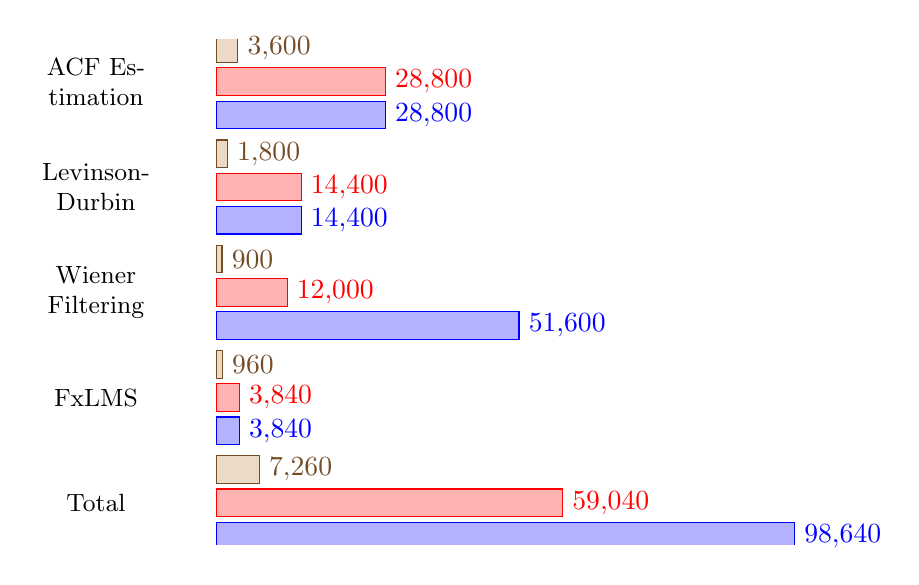
\begin{tikzpicture}
  \begin{axis}[
    width  = 0.85*\textwidth,
    height = 8cm,
    xbar,
    y axis line style = { opacity = 0 },
    axis x line       = none,
    tickwidth         = 0pt,
%    enlarge y limits  = 0.2,
%    enlarge x limits  = 0.02,
    y tick label style={font=\small,text width=1.5cm,align=center},
    symbolic y coords = {Total,FxLMS, Wiener Filtering, Levinson-Durbin, ACF Estimation},
    nodes near coords,
  ]
  \addplot coordinates {(98640,Total) (3840,FxLMS)         (51600,Wiener Filtering)
                         (14400,Levinson-Durbin)  (28800,ACF Estimation) };
  \addplot coordinates {(59040,Total) (3840,FxLMS)         (12000,Wiener Filtering)
                         (14400,Levinson-Durbin)  (28800,ACF Estimation) };
  \addplot coordinates {(7260,Total) (960,FxLMS)         (900,Wiener Filtering)
                         (1800,Levinson-Durbin)  (3600,ACF Estimation) };
  \end{axis}
\end{tikzpicture}
}
		\end{center}
	
		\end{column}
	\end{columns}

\end{frame}

% \subsection{Multirate}
% \begin{frame}{Implementation Consideration}{Multirate}

% 	\begin{columns}
% 		\begin{column}{0.4\textwidth}
% \begin{itemize}
% \item Reduce to computation demands N-fold
% \begin{itemize}
% \item Lower prediction length
% \item 12 kHz is a factor $2^4$ lower in computation cost 
% \end{itemize}
% \end{itemize}
% Procedure: 
% \begin{enumerate}
% \item Downsample from 192 kHz to 12 kHz
% \begin{itemize}
% \item Decimate by an order of 2
% \item 1$^{st}$ IIR filter 
% \end{itemize}
% \item Perform  prediction
% \item Upsample from 12 kHz to 192 kHz
% \begin{itemize}
% \item Upsampling by order of 2 
% \item 1$^{st}$ IIR filter 
% \end{itemize}
% \end{enumerate}
% 		\end{column}
% 		\begin{column}{0.6\textwidth} 
		
% 		\begin{center}
% \begin{table}[]
% \centering
% \begin{tabular}{|c|c|c|c|c|c|}
% \hline
% $fs$                                                          & 192 & 96 & 48 & 24 & 12 \\ \hline
% \begin{tabular}[c]{@{}c@{}}Prediction\\ Length\end{tabular}   & 43  & 22 & 11 & 6  & 3  \\ \hline
% \end{tabular}
% \end{table}


% \resizebox{1\columnwidth}{!}{	
% \begin{tikzpicture}
%   \begin{axis}[
%     width  = 0.85*\textwidth,
%     height = 6cm,
%     xbar,
%     y axis line style = { opacity = 0 },
%     axis x line       = none,
%     tickwidth         = 0pt,
%     enlarge y limits  = 0.2,
%     enlarge x limits  = 0.02,
%     y tick label style={font=\small,text width=1.5cm,align=center},
%     symbolic y coords = {FxLMS, Wiener Filtering, Levinson-Durbin, ACF Estimation},
%     nodes near coords,
%   ]
%   \addplot coordinates { (57727,FxLMS)         (5672,Wiener Filtering)
%                          (2193,Levinson-Durbin)  (11106,ACF Estimation) };
%   \addplot coordinates { (57727,FxLMS)         (5672,Wiener Filtering)
%                          (2193,Levinson-Durbin)  (11106,ACF Estimation) };
% %  \legend{Topics, Posts}
%   \end{axis}
% \end{tikzpicture}
%  }


% 		\end{center}
	
% 		\end{column}
% 	\end{columns}




% \end{frame}









\begin{frame}{Discussion}{General}		
\begin{itemize}
	\item Single person vs multiple persons
	\begin{itemize}
		\item ACF changes 
	\end{itemize}
	\item Varying perfomance
\end{itemize}
\end{frame}

\section{Conclusion}
\begin{frame}{Conclusion}{General}		
\begin{itemize}
	\item Proof of concept
	\item System
	\begin{itemize}
		\item Linear Prediction
		\item Feedforward FXLMS
	\end{itemize}
	\item Only tested for single person
	\item Increased attenuation of up to 34 dB
\end{itemize}
\end{frame}

\begin{frame}{Conclusion}{Computational Cost}		
\begin{itemize}
\item Computational cost of system (instructions per sample) = 98640
	\begin{itemize} 
		\item $f_s = 48$ [kHz]
		\item P = 43: 
		\item N = 1200
		\item O = 1100
	\end{itemize}
\item Computational cost of system (instructions per sample) = 59040
	\begin{itemize}
		\item $f_s = 48$ [kHz]
		\item P = 10: 
		\item N = 1200
		\item O = 1100
	\end{itemize}
\item Computational cost of system (instructions per sample) = 7260
	\begin{itemize}
		\item $f_s = 12$ [kHz]
		\item P = 3: 
		\item N = 300
		\item O = 250
	\end{itemize}
\end{itemize}
\end{frame}